\documentclass[10pt]{article}
\usepackage[utf8]{inputenc}
\usepackage[T1]{fontenc}
\usepackage{amsmath}
\usepackage{amsfonts}
\usepackage{amssymb}
\usepackage[version=4]{mhchem}
\usepackage{stmaryrd}
\usepackage{hyperref}
\hypersetup{colorlinks=true, linkcolor=blue, filecolor=magenta, urlcolor=cyan,}
\urlstyle{same}
\usepackage{graphicx}
\usepackage[export]{adjustbox}
\graphicspath{ {./images/} }
\usepackage{bbold}

\title{Recommended Citation }


\author{A Wave-Adaptive Modular Vessel (WAM-V) is an under- actuated system. There are\\
fewer control inputs than the numbers of the degree of freedom. Control of a WAM-V is\\
challenging due to its underactuated nature. In oceans, there are unknown currents applied to a\\
WAM-V. Therefore, in the model of a WAM-V, there are disturbances. Considering the\\
complexity of tasks, robustness and flexibility of multiple WAM-Vs, coordination of multiple\\
systems has been an important mission. We considered formation control of multiple WAM-Vs\\
with uncertainty. There are parametric uncertainty and non-parametric uncertainty in the model\\
of each WAM- V and the information of the leader WAM-V is available only to a portion of the\\
follower WAM-Vs. In this chapter, we consider formation control of multiple WAM-Vs with\\
uncertainty and a leader vehicle. Distributed robust controllers are proposed with the aid of\\
adaptive backstepping techniques. The proposed control laws ensure that the formation errors\\
and the tracking errors exponentially converge to zero. To reduce the computation load in\\
controller design, distributed command filtered controllers are proposed. To verify the\\
effectiveness of the proposed cooperative control laws, simulation results are presented.}
\date{}


\begin{document}
\maketitle
University of Texas Rio Grande Valley

ScholarWorks @ UTRGV

Theses and Dissertations

$5-2021$

Robust Distributed Formation Control of UAVs with Higher-Order

Dynamics

Md Nur-A-Adam Dony

The University of Texas Rio Grande Valley

Follow this and additional works at: \href{https://scholarworks.utrgv.edu/etd}{https://scholarworks.utrgv.edu/etd}

Part of the Electrical and Computer Engineering Commons

Dony, Md Nur-A-Adam, "Robust Distributed Formation Control of UAVs with Higher-Order Dynamics" (2021). Theses and Dissertations. 856.

\href{https://scholarworks.utrgv.edu/etd/856}{https://scholarworks.utrgv.edu/etd/856}

This Thesis is brought to you for free and open access by ScholarWorks @ UTRGV. It has been accepted for inclusion in Theses and Dissertations by an authorized administrator of ScholarWorks @ UTRGV. For more information, please contact \href{mailto:justin.white@utrgv.edu}{justin.white@utrgv.edu}, \href{mailto:william.flores01@utrgv.edu}{william.flores01@utrgv.edu}. ROBUST DISTRIBUTED FORMATION CONTROL OF UAVS

WITH HIGHER-ORDER DYNAMICS

May 2021

Major Subject: ELECTRICAL ENGINEERING

\section*{ROBUST DISTRIBUTED FORMATION CONTROL OF UAVS WITH HIGHER-ORDER DYNAMICS }


\section{COMMITTEE MEMBERS}
Dr. Wenjie Dong Chair of Committee

Dr. Jun Peng

Committee Member

Dr. Weidong Kuang Committee Member

May 2021 Copyright 2021 MD NUR-A-ADAM DONY

All Rights Reserved

\begin{abstract}
Md Nur-A-Adam, Dony, Robust Distributed Formation Control of UAVs with $\underline{\text { Higher-Order }}$ Dynamics. Master of Science in Engineering (MSE); May 2021, 57 pp., 13 figures, 22references.
In this thesis, we introduce distributed formation control strategies to reach an intended linear formation for agents with a diverse array of dynamics. The suggested technique is distributed entirely, does not include inter-agent cooperation or a barrier of orientation, and can be applied using relative location information gained by agents in their local cooperation frames. We illustrate how the control optimized for agents with the simpler dynamic model, i.e., the dynamics of the single integrator, can be expanded to holonomic agents with higher dynamics such as quadrotors and non-holonomic agents such as unicycles and cars. Our suggested approach makes feedback saturations, unmodelled dynamics, and switches stable in the sensing topology. We also indicate that the control is relaxed as agents will travel along with a rotated and scaled control direction without disrupting the convergence to the desired formation. We can implement this observation to design a distributed strategy for preventing collisions. In simulations, we explain the suggested solution and further introduce a distributed robotic framework to experimentally validate the technique. Our experimental platform is made up of off-the-shelf devices that can be used to evaluate other multi-agent algorithms and verify them.
\end{abstract}

\section{DEDICATION}
The completion of my master's studies would not have been possible without the love and support of my family. Thank you for your love and patience.

\section{ACKNOWLEDGEMENTS}
I will always be grateful to Dr. Wenjie Dong, chair of my thesis committee, for all his mentoring and advice. He encouraged me to complete this process through his infinite patience

and guidance. My thanks go to my thesis committee members: Dr. Weidong Kuang, and Dr. Jun Peng. Their advice, input, and comments on my dissertation helped to ensure the quality of my intellectual work. I would also like to thank my colleagues at the UTRGV library who helped me locate supporting documents for my research. Work in this thesis is based upon the grant UTRGV Presidential Graduate Research Assistant (PGRA) scholarship funding.

\section{TABLE OF CONTENTS}
\section{Page}
\begin{center}
\includegraphics[max width=\textwidth]{2023_10_07_53b70c7408bc8e139415g-14(2)}
\end{center}

\begin{center}
\includegraphics[max width=\textwidth]{2023_10_07_53b70c7408bc8e139415g-14(5)}
\end{center}

\begin{center}
\includegraphics[max width=\textwidth]{2023_10_07_53b70c7408bc8e139415g-14(1)}
\end{center}

\begin{center}
\includegraphics[max width=\textwidth]{2023_10_07_53b70c7408bc8e139415g-14(11)}
\end{center}

\begin{center}
\includegraphics[max width=\textwidth]{2023_10_07_53b70c7408bc8e139415g-14(3)}
\end{center}

\begin{center}
\includegraphics[max width=\textwidth]{2023_10_07_53b70c7408bc8e139415g-14}
\end{center}

\begin{center}
\includegraphics[max width=\textwidth]{2023_10_07_53b70c7408bc8e139415g-14(10)}
\end{center}

\begin{center}
\includegraphics[max width=\textwidth]{2023_10_07_53b70c7408bc8e139415g-14(7)}
\end{center}

1.3 Motivation and Applications..........................................................

1.4 Formation Control and Related Work................................................

\begin{center}
\includegraphics[max width=\textwidth]{2023_10_07_53b70c7408bc8e139415g-14(6)}
\end{center}

CHAPTER II. FORMATION CONTROL AND GUIDANCE OF UAVS AT CONSISTENT

\begin{center}
\includegraphics[max width=\textwidth]{2023_10_07_53b70c7408bc8e139415g-14(9)}
\end{center}

\begin{center}
\includegraphics[max width=\textwidth]{2023_10_07_53b70c7408bc8e139415g-14(4)}
\end{center}

2.2 Formation Control for Single Integrator Dynamics..................................10

\begin{center}
\includegraphics[max width=\textwidth]{2023_10_07_53b70c7408bc8e139415g-14(8)}
\end{center}

2.4 Formation Control Without Input Constraints

2.5 Formation Control with Input Constraints..........................................18

\begin{center}
\includegraphics[max width=\textwidth]{2023_10_07_53b70c7408bc8e139415g-15(3)}
\end{center}

2.7 Concluding Remarks and Future Work........................................23

CHAPTER III. VIGOROUS PLANAR FORMATION CONTROL FOR HIGHER-ORDER

\begin{center}
\includegraphics[max width=\textwidth]{2023_10_07_53b70c7408bc8e139415g-15(5)}
\end{center}

3.1 Notation and Assumptions.....................................................26

3.2 Problem statement.........................................................26

3.3 Robustness to Perturbations.................................................27

3.4 Formation Control for Agents with Higher-Order Dynamics........................28

\begin{center}
\includegraphics[max width=\textwidth]{2023_10_07_53b70c7408bc8e139415g-15(2)}
\end{center}

3.6 Concluding Remarks and Future work......................................35

CHAPTER IV. DISTRIBUTED COMMAND FILTERED ROBUST TRACKING CONTRO L OF WAVE-ADAPTIVE MODULAR VESSEL WITH UNCERTAINTY ...............36

4.1 Problem Statement........................................................ 37

4.2 Distributed Robust Controller Design..........................................39

4.3 Distributed Command Filtered Tracking Control Laws..........................45

\begin{center}
\includegraphics[max width=\textwidth]{2023_10_07_53b70c7408bc8e139415g-15(4)}
\end{center}

\begin{center}
\includegraphics[max width=\textwidth]{2023_10_07_53b70c7408bc8e139415g-15}
\end{center}

CHAPTER V. CONCLUSION AND FUTURE RESEARCH............................53

\begin{center}
\includegraphics[max width=\textwidth]{2023_10_07_53b70c7408bc8e139415g-15(1)}
\end{center}

BIOGRAPHICAL SKETCH...............................................................

\section{LIST OF FIGURES}
Page

Figure 2.1: Simulation of 9 UAVs starting from a random initial pose and achieving a square formation while traveling along toward the positive x-axis. (a)Initial pose at (a)t=0s. (b) $t=52 s$. (c) $t=100 s$. (d) $t=192 \mathrm{~s}$.

Figure 2.2: Simulation of 9 UAVs starting from a random initial pose and achieving a square formation with fixed scale while traveling along toward the positive x-axis. Initial pose at (a)t=0s. (b) $t=52$ s. (c) $t=100$ s. (d) $t=192$ s...............20

Figure 2.3: Simulation of 6 UAVs starting from a random initial pose and achieving a triangle formation while traveling along toward the positive $\mathrm{x}$-axis. Initial po

\begin{center}
\includegraphics[max width=\textwidth]{2023_10_07_53b70c7408bc8e139415g-16}
\end{center}

Figure 2.4: Simulation of 6 UAVs starting from a random initial pose and achieving a triangle formation while traveling along toward the positive $\mathrm{x}$-axis. Initial pose at (a)t $=0$ s. (b) $t=31$ s. (c) $t=63 s$. (d) $t=102 s$

Figure.3.1: Simulation of 9 quadrotors with a square grid desired formation (actual size of vehicles increased by a factor of 1.6 for better visibility). (a) Top view at (a)t $=0 \mathrm{~s}(\mathrm{~b}) \mathrm{t}=17 \mathrm{~s}$. (c) $\mathrm{t}=29 \mathrm{~s}$. (d) $\mathrm{t}=40 \mathrm{~s}$.

Figure 3.2: Simulation of 9 unicycles with a square grid desired formation (actual size of vehicles increased by a factor of 1.5 for better visibility). Top view at (a)t $=0$ s. (b) $t=6 s$. (c) $t=9 s$. (d) $t=15$ s. Figure 4.1: Desired formation of three WAM-Vs

Figure 4.2: Communication digraph .............................................49

\begin{center}
\includegraphics[max width=\textwidth]{2023_10_07_53b70c7408bc8e139415g-17}
\end{center}

\begin{center}
\includegraphics[max width=\textwidth]{2023_10_07_53b70c7408bc8e139415g-17(1)}
\end{center}

\begin{center}
\includegraphics[max width=\textwidth]{2023_10_07_53b70c7408bc8e139415g-17(4)}
\end{center}

\begin{center}
\includegraphics[max width=\textwidth]{2023_10_07_53b70c7408bc8e139415g-17(3)}
\end{center}

\begin{center}
\includegraphics[max width=\textwidth]{2023_10_07_53b70c7408bc8e139415g-17(2)}
\end{center}

\section{CHAPTER I}
\section{INTRODUCTION}
\subsection{General Introduction}
In recent years, technological innovations have found it incredibly feasible to mobilize a vast number of agents to conduct activities cooperatively, such as environmental mapping and monitoring (Keller et al., 2017; Thomas et al.2001;Tanner et al.,2001) distribution of goods, and manipulation of objects. The ability to get the agents to a desired geometric form in this implementation is a fundamental component (Leonard and Fiorelli,2001) By using this ability, we will be able to design more advanced strategies for maneuvering and navigation. Distributed formation control strategies guarantee that a desired geometric shape emerges from agents' collective actions by appointing local control laws to individual agents. Distributed techniques provide greater scalability relative to clustered approaches. They also arrange automatically parallelized computing, tolerance to connectivity interruption and hardware malfunction, robustness to instability, absence of global measurements.

We propose a coherent distributed control strategy for planar agent formations with a range of dynamics in this work. In specific, we consider agents with linear or linearizable rigidbody dynamics such as quadrotors. Then the control is further applied to agents with non holonomic dynamics such as Cars and unicycles. To evaluate control gains for agents with the single-integrator model, we begin by constructing a semidefinite programming (SDP) problem. We demonstrate robustness characteristics in this design approach such as Robustness to input saturation, topology switching in the sensing, and disruptions in the direction of control. Control of single-integrator agents is gradually added to agents. For higher-order holonomic dynamics, it is possible to explicitly use the collection of control gains determined from the SDP problem to accomplish the formation without having to reinvent the control. Several models are presented to validate the theoretical findings. Quadrotors, differential drive robots with singlecycle mechanics, and vehicles, where it is shown that the agents obtain the desired outcomes.

\subsection{Literature Review}
There exists a large body of work on formation control of multi-agent systems (J. C. Barca and Y. A. Sekercioglu,2013) however, depending on the restrictions and assumptions considered in the problem, existing literature can be divided into smaller categories. Examples are classes of methods that require position measurements in a global coordinate frame (Michael et al., 2008; Hyun et al.,2016) a common heading direction Montijano et al., 2014; Zhou et al.,2015) inter-agent communication (Park et al., 2017; Weinstein et al.,2018), or a complete inter-agent sensing graph (Aranda et al., 2015) Unlike the aforementioned methods, a certain class of formation control strategies do not require these assumptions, and a desired formation can be achieved without global measurements or communication. Distance-based (Saber et al., 2017; Krick et al.,2009; Taian et al.,2013) bearing-based (Wang et al., 2014; Fathian et al.,2016; Wang et al.,2016) formation control strategies are among the methods that fall in the latter class. In a barycentric coordinate-based formation control strategy, in contrast to distance- and bearingbased formations, the desired formation is defined in terms of both distances and bearing angles that are subtended from agents to their neighbors. Since common sensors such as laser scanners, radars, sonars, and stereo cameras can provide both angle and distance measurements, the focus of this work is such desired formations.

\subsection{Motivation and Applications}
\subsubsection{Unmanned Aerial Vehicles}
An Unmanned Aerial Vehicle (UAV) is known as a powered flying vehicle that does not carry a human operator, that can be operated remotely or autonomously and that can carry a payload. The UAVs can be used in both military and civilian applications. UAVs can carry out tasks without placing human pilots in jeopardy. Additionally, UAVs can operate in hazardous conditions or require tedious or onerous piloting during lengthy operations. Different types of Unmanned Aerial Vehicles (UAVs) have become available in recent years, namely, fixed-wing UAVs and rotary-wing UAVs. Compared with fixed-wing UAVs, the rotary-wing UAVs have advantages such as Vertical Taking Off and Landing (VTOL) ability. The rotary-wing UAVs cover helicopters and multirotors. A multirotor is a rotorcraft with more than two rotors. Compared to helicopters, a multirotor has the simplicity of rotor mechanics required for flight control. Unlike conventional helicopters, which are mechanically very complex, the multirotor usually uses fixed-pitch blades. The control of vehicle motion is achieved by varying the relative speed of each rotor in order to change the thrust and torques. VTOL, Quadrotors also have advantages such as maneuverability, low-cost, small size, and easy handling. These advantages motivate researchers to pay attentions on quadrotors. Other advantages of quadrotors are reliability and compactness, which are essential for a system that will be portable and useful in close proximity to people and structures for commercial applications.

\subsection{Formation Control \& Related Work}
The formation control of a multi-UAV system is an important category of networked systems due to their commercial and military applications. The control objective of the formation of multiple quadrotors contains the consensus and the formation pattern of the quadrotors. According to the different requirements on the patterns, the formation can be divided into two types, which are the rigid and flexible formations.

\subsubsection{Consensus}
A general definition of consensus is given in the literature such as the one in Olfati-Saber al., et 2007 | Olfati-Saber and Murray, 2004 |Saber and Murray, 2003a :"In networks of agents or dynamic systems, consensus means to reach an agreement regarding a certain quantity of interest that depends on the state of all agents". The consensus problems can be classified by "unconstrained consensus problems" and "constrained consensus problems". an objective function exists such that the state of all agents has to asymptotically become equal to this function, while in an unconstrained consensus problem, it is sufficient that the state of all agents asymptotically be the same without computing any objective function. For example, in a multivehicle system, an unconstrained consensus is achieved, if the goal of each vehicle is to minimize its local cost as follows

$$
U_{i}(x)=\Sigma_{j \in \mathcal{N}_{i}}\left\|x_{j}-x_{i}-d_{i j}\right\|^{2}
$$

where $x_{i}$ is the position of vehicle $i$ and $d_{i j}$ is a desired inter-vehicle relative-position vector. Vehicle $j$ is the neighbor of vehicle $i$.

\subsubsection{Leader-Follower formation configuration}
The leader-follower, virtual leader and behavior-based configurations are seen in the literature. The formation control of multi-agent systems using the Leader Follower (L-F) configuration is particularly attractive due to its simplicity and scalability | Roldao et al., 2014.Within the L-F configuration, some agents are designated as leaders while others are treated as followers. The states of the leader constitute the coordination variable, since the actions of the other in the formation are completely specified once the leader states are known Montenegro et al., 2014, ||Ren et al., 2005. The L-F configuration has the advantage of simplicity, since the moving trajectory of the flock is clearly given to the leader(s) |Fax and Murray, 2004.Then, the followers follow the leader(s) to keep the formation. Compared to the "behavior-based" approach, the L-F configuration is efficient and simple for applications in practice I Hou and Fantoni, 2015a. In the "behavior-based" approach without leader, the agent in the flock usually has random behaviors to overcome local maxima or minima | Balch and Arkin, \href{http://1998.In}{1998.In} the standard L - F formation configuration, the leader can affect the followers whenever it is in their neighboring set but there is no feedback from the followers to the leader. Such works can be found in papers | Ni and Cheng, 2010,| Hong et al., 2006 |, Ji et al., 2009, where the leader is treated as a special agent whose motion is independent on other agents.

The first advantage is the efficiency. the searching trajectory is clearly specified by the leader(s), while the followers keep around the leader(s) for the purpose of extending the searching scope of the leader(s). Furthermore, the L-F configuration is considered as an energy saving mechanism | Ni and Cheng, 2010 and ||Hummel, 1995. Additionally, the L-F formation configuration can avoid "information-based instability" according to John Baillieul and Panos J. Antsaklis |Baillieul and Antsaklis, 2007.

\subsection{Contributions of This Dissertation}
In this work, we present a unified distributed control strategy for planar formations of agents with a variety of dynamics. In particular, we consider agents with linear or linearizable holonomic dynamics, such as quadrotors, and further extend the control to agents with nonholonomic dynamics such as unicycles and cars. We start by formulating a semidefinite programming (SDP) problem to determine control gains for agents with the single-integrator model. We show that this design strategy enjoys several robustness properties such as robustness to saturations in the input, switching in the sensing topology, and disturbances in the control direction. We show that if agents move along a control direction that is scaled by an arbitrary positive value, and rotated by, an arbitrary amount up to $\pm 90^{\circ}$, convergence to the desired formation is still guaranteed. This observation is exploited later to design a fully distributed collision avoidance strategy. The control for single-integrator agents is extended subsequently to agents with higher-order holonomic dynamics, where we show the set of control gains computed from the SDP problem can be used directly to achieve the formation without having to redesign the control. As an example, we use the gains designed for single-integrator agents to achieve a planar formation of quadrotors. Following the same philosophy, we show that the control gains can be used directly for agents with nonholonomic dynamics such as unicycles and cars.

Furthermore, the proposed nonholonomic control remains robust to input saturations and unmodeled/unknown dynamics. To vet the theoretical results, several simulations are presented for quadrotors, differential drive robots with unicycle dynamics, and cars, where it is shown that agents achieve a desired formation without collision. To typify the results further, the proposed control strategy is tested experimentally on a distributed differential-drive wheeled robotic platform with different numbers of robots and desired formations. In summary, the main contributions are

\begin{itemize}
  \item A distributed planar formation control for vehicles with a large variety of holonomic and nonholonomic dynamics.

  \item Eliminating the need for global position measurements, common heading direction, interagent communication, or complete sensing graph.

  \item Guaranteed global convergence to the desired formation with provable robustness to saturated input, unmodeled dynamics, and disturbances.

  \item A fully distributed and heuristic collision avoidance algorithm incorporated in the formation control strategy.

  \item A low-cost distributed robotic platform with off-the shelf components for validation of distributed control algorithms.

\end{itemize}

\section{CHAPTER II}
\section{FORMATION CONTROL AND GUIDANCE OF UAVS AT CONSISTENT ELEVATION}
In this work, we propose a distributed guidance strategy to navigate a team of fixed-wing UAVs at a constant altitude toward a desired waypoint. Our strategy is based on using the unicycle kinematic model for UAVs' motion, where the airspeed and turning rate of UAVs must satisfy practical bounds known as the Dubins constraints as one in Fathian et al., 2016. Given a set of control gains and a desired destination, which can be communicated to the agents before the mission, onboard sensor measurements of each UAV can be used to compute a control direction. This control is well-suited as a high-level motion planning input to a low-level UAV autopilot, which can compensate for the aerodynamics, wind effects, disturbances, etc., that are not accounted for in the unicycle model. Advantages of the proposed strategy over centralized methods include better scalability, naturally parallelized computation, resilience to communication loss and hardware failure, and robustness to uncertainty and lack of global knowledge. In particular, the UAVs can achieve the formation using only the local relative position measurements of their neighbors, and without communicating with each other. This increases the stealth and robustness of the team to jamming. Simulations are presented to typify the performance of the proposed strategy.

\subsection{Problem statement}
In recent years, the Unmanned Aerial Vehicle (UAV) technology has reached a level of maturity that it is now possible to deploy hundreds of UAVs in a mission. The large number of deployed vehicles allows a team of small, inexpensive UAVs to efficiently execute missions such as search and rescue inspection and surveillance. As the number of deployed UAVs increases, controlling agents from a command center becomes less practical. This is due to the limited communication bandwidth, which becomes saturated as the number of agents increases. Furthermore, the centralized control lacks resilience to communication loss, hardware failure, and malicious attacks such as jamming or spoofing of the communication signal. Hence, UAVs in large teams should have a level of autonomy to individually plan their motion in accordance with the team to perform the desired task. To navigate the UAVs between waypoints, distributed formation -control techniques can be employed, where the UAVs autonomously achieve a desired formation and travel toward the desired destination. We present a distributed control strategy for a team of fixed-wing Unmanned Aerial Vehicles (UAVs), such that they achieve a desired formation and travel along a desired direction at a constant altitude. We describe the motion of UAVs with the kinematic unicycle model. Based on this model, a control strategy is proposed, and local convergence of the team to the desired formation and travel direction is proved. The control direction returned by our strategy is well-suited, which can compensate for the aerodynamics, wind effects, disturbances, etc., that are not accounted for in the unicycle model.

The proposed strategy is fully distributed and can be implemented using relative position measurements acquired by UAVs in their local coordinate frames. Furthermore, UAVs do not need to communicate. Simulations are provided to typify the proposed strategy.

\subsection{Formation Control for Single-Integrator Dynamics}
In this section, we present the distributed formation control strategy introduced in (Lin et al.,2014), for agents with single-integrator dynamics. We then propose a novel design approach for finding stabilizing control gains by formulating a convex optimization problem. The results of this section are a cornerstone for formation control of agents with more complicated dynamic models that are discussed in the subsequent sections.

\subsubsection{Control strategy}
The single-integrator dynamics can be described as

$$
\dot{q}_{i}=u_{i}
$$

where $q_{i}:=\left[x_{i}, y_{i}\right]^{\top} \in \mathbb{R}^{2}$ is the coordinate of agent $i \in\{1,2 \ldots, n\}$ in a common global coordinate frame (unknown to the agent), and $u_{i} \in \mathbb{R}^{2}$ is the control law. To bring the agents to a desired formation, the control law for each agent can be chosen as

$$
u_{i}:=\sum_{j \in \mathcal{N}_{i}} A_{i j}\left(q_{j}-q_{i}\right)
$$

where $A_{i j} \in \mathbb{R}^{2 \times 2}$ are constant control gain matrices that will be designed later, and each has the form

$$
A_{i j}:=\left[\begin{array}{cc}
a_{i j} & b_{i j} \\
-b_{i j} & a_{i j}
\end{array}\right], a_{i j}, b_{i j} \in \mathbb{R}
$$

Thanks to the commutativity property of the $A_{i j}$ matrices, the closed-loop dynamics with coordinates $q_{i}$ and $q_{j}$ expressed in agents' local coordinate frames is identical to the case that coordinates are expressed in a global coordinate frame. The geometric intuition behind the control strategy (3.2) is explained in the following example. Example 1 .Consider three agents in Fig. 2, where agents 2 and 3 are neighbors of agent 1 .Let $q_{2}=[2,3]^{\top}$ and $q_{3}=[3,1]^{\top}$ denote the position of neighbors in agent 1's local coordinate frame, and assume that control gains for agent 1 are given as

$$
A_{12}=\left[\begin{array}{cc}
2 & -1 \\
1 & 2
\end{array}\right], A_{13}=\left[\begin{array}{cc}
-1 & 3 \\
-3 & -1
\end{array}\right]
$$

From (2), the control vector for agent 1 is computed as

$$
u_{1}=A_{12} q_{2}+A_{13} q_{3}=\left[\begin{array}{c}
1 \\
-2
\end{array}\right]
$$

which is shown in the figure and can be interpreted geometrically as follows. At any instance of time, agent 1 moves along the control vector with the speed equal to the vector's magnitude. Note that due to the special structure of gain matrices $A_{12}, A_{13}$, they can be interpreted as scaled rotation matrices that rotate and scale vectors connecting agent 1 to its neighbors. One can see that this action is independent of agent 1's local coordinate frame position and orientation, hence, $q_{1}$ and $q_{2}$ can replaced by their coordinates in a global coordinate frame for analysis.

Let $q:=\left[q_{1}^{\top}, q_{2}^{\top}, \ldots, q_{n}^{\top}\right]^{\top} \in \mathbb{R}^{2 n}$ and $u:=\left[u_{1}^{\top}, u_{2}^{\top}, \ldots, u_{n}^{\top}\right]^{\top} \in \mathbb{R}^{2 n}$ denote the aggregate state and control vectors of all agents, respectively. he closed-loop dynamics under the control strategy (2.2) can be expressed as, $\quad \grave{q}=A q$

$$
A=\left[\begin{array}{cccc}
-\sum_{j=2}^{n} A_{1 j} & A_{12} & \cdots & A_{1 n} \\
A_{21} & -\sum_{j=1}^{n} A_{2 j} & \cdots & A_{2 n} \\
& j \neq 2 & & \\
\vdots & & \ddots & \vdots \\
A_{n 1} & A_{n 2} & \cdots & -\sum_{j=1}^{n-1} A_{n j}
\end{array}\right]
$$

where for $j \notin \mathcal{N}_{i}$ the $A_{i j}$ block is defined as a zero matrix. Note that the $2 \times 2$ diagonal blocks of $A$ are the negative sum of the rest of the blocks on the same row. Hence, $A$ has block Laplacian structure, and it follows that vectors

$$
\begin{aligned}
& \mathbf{1}:=[1,0,1,0, \ldots, 1,0]^{\top} \in \mathbb{R}^{2 n} \\
& \overline{\mathbf{1}}:=[0,1,0,1, \ldots, 0,1]^{\top} \in \mathbb{R}^{2 n}
\end{aligned}
$$

are in the kernel ${ }^{1}$ of $A$. Let $q^{*} \in \mathbb{R}^{2 n}$ denote the coordinates of agents at the desired formation (the orientation, translation, and scale of the desired formation can be chosen arbitrarily). Further, let $\hat{q}^{*} \in \mathbb{R}^{2 n}$ denote the coordinates of agents when the desired formation is rotated by 90 degrees about the origin. The following theorem states the conditions that guarantee the convergence of agents to the desired formation.

Theorem 1. Fathian et al., 2016 Considered agents with single-integrator dynamics (2.1) and control (2.2). If the $\mathrm{A}_{i j}$ 's are chosen such that, (i) $A$ has null vectors $\mathbf{1}, \overline{\mathbf{1}}, q^{*}$ and $\bar{q}^{*}$, (ii) Other than the four zero eigenvalues associated with these null vectors, all eigenvalues of A have negative real parts, then, agents globally converge to the desired formation.

Note that in Theorem 1 convergence to the desired formation implies that the formation is achieved up to a rotation and translation in the global coordinate frame, and a non-negative scale factor. As we will discuss in Section VII, in applications where the scale is important, the control can be augmented to attain the desired scale. We should point out that null vectors $\mathbf{1}, \overline{\mathbf{1}}$ correspond to the case where all agents coincide, which can be interpreted as the desired formation achieved with the zero scale. It can be shown that the set of initial conditions that converge to this coinciding equilibrium is measure zero. Notice that in practice, trajectories of agents cannot remain on a measure zero set (due to noise, disturbances, etc.), thus, coinciding agents are not of practical concern.

Remark 1. The topological conditions that guarantee the existence of a symmetric matrix A satisfying the conditions of Theorem 1 are studied in (Z. Lin et al.2016), which presents the necessary and sufficient condition that the sensing graph is undirected and universally rigid. Throughout this paper, we assume that this condition is met.

\subsubsection{Control Gain Design}
Given a desired formation for agents with a universally rigid sensing topology, we present a novel algorithm to find control gain matrices that meet the conditions of Theorem 1. Let $N:=\left[q^{*}, \bar{q}^{*}, \mathbf{1}, \overline{\mathbf{1}}\right] \in \mathbb{R}^{2 n \times 4}$ be the set of bases for the kernel of $A$, where $1, \overline{1}$ are given in (7), $q^{*} \in \mathbb{R}^{2 n}$ is the coordinates of agents at the desired formation, and $\bar{q}^{*} \mathbb{R}^{2 n}$ is the $90^{\circ}$ rotated coordinates about the origin. Let $U S V^{\top}=N$ be the (full) singular value decomposition (SVD) of $N$, where

$$
U=[\bar{Q}, Q] \in \mathbb{R}^{2 n \times 2 n}
$$

with $Q \in \mathbb{R}^{2 n \times(2 n-4)}$ defined as the last $2 n-4$ columns of $U$.

Lemma 1. Using $Q$ in (8), define

$$
\bar{A}:=Q^{\top} A Q \in \mathbb{R}^{(2 n-4) \times(2 n-4)}
$$

Matrices $A$ and $\bar{A}$ have the same set of nonzero eigenvalues.

Proof of Lemma 1 follows by observing that $U$ is an orthogonal matrix, and range $(\bar{Q})=$ range $(N)$. Therefore $\bar{A}$ is the projection of $A$ onto the orthogonal complement of range $(N)$. Effectively, the projection operation in (9) removes the zero eigenvalues of $A$. For an undirected sensing topology, by imposing the constraints $a_{i j}=a_{j i}, b_{i j}=-b_{j i}$ in (3) matrix $A$ can be designed to be symmetric. Note that from Remark 1 existence of such matrix is guaranteed. In this case, $\bar{A}$ is symmetric, and its eigen values are real and can be ordered. Hence, $A$ can be computed by solving the optimization problem

$$
\begin{array}{cc}
A=\underset{a_{i j}, b_{i j}}{\operatorname{argmax}} & \lambda_{1}(-\bar{A}) \\
\text { subject to } & A N=0
\end{array}
$$

\section{Algorithm 1: Formation control gain design.}
input: Desired formation coordinates $q^{*}$

output: Gain matrix A.

step 1: Let $\mathrm{N}:=\left[q^{*}, \hat{q}^{*}, \mathbf{1}, \overline{\mathbf{1}}\right]$

step 2: Compute SVD of $\mathrm{N}=U S V^{\top}$.

step 3: Define $\mathrm{Q}$ as the last 2n-4 columns of $\mathrm{U}$.

step 4: Solve (2.10) using SDP solver.

where $\lambda_{1}(\cdot)$ denote the smallest eigenvalue of a matrix. Note that (10) is a concave maximization problem and can be formulated as the SDP problem

$$
\begin{aligned}
A=\operatorname{argmax} & \gamma \\
a_{i j}, b_{i j}, \gamma & \\
\text { subject to } & \bar{A}+\gamma I \preceq 0 \\
& A N=0
\end{aligned}
$$

where the first constraint is a linear matrix inequality. In recent years, effective algorithms for numerically solving SDPs have been developed and are now available (R. H. Tütüncü et al.2003). The proposed approach for finding stabilizing gain matrix $A$ is summarized in Algorithm 1.

We point out that the optimization approach used here relies on a centralized paradigm and knowledge of the sensing topology. Once gains are computed, they can be transmitted to agents before the mission.If agents can communicate, distributed optimization techniques can be used to solve (2.11) without relying on the complete knowledge of the sensing topology.

\subsection{Formation Control for UAVS}
In this section, we introduce the unicycle kinematic model with Dubins constraints, which provides a good description of the UAV's motion that is well suited for a high-level path planning autopilot control input. Based on this model, we develop a guidance strategy for UAVs such that they autonomously achieve a desired formation and travel along a straight line toward a desired destination.

We first propose a strategy without enforcing the Dubins constraints on the speed and rate of turn of aircrafts. We then extend the control to include the Dubins constraints. Throughout this section, we assume that the sensing graph is undirected, and a symmetric negative semi-definite control gain matrix $A$ is designed for the desired formation by solving the optimization problem.

\subsubsection{Unicycle Kinematic Model with Dubins Constraints}
Under the assumption that the autopilot is tuned to set the airspeed and heading angle of a UAV to desired commanded values, the unicycle kinematic model provides a good description of the UAV's motion at a constant altitude. In (2.12), $x_{i}, y_{i} \in \mathbb{R}$ are coordinates of agent $i$.

$$
\begin{aligned}
\grave{x}_{i} & =v_{i} \cos \left(\theta_{i}\right) \\
\grave{y}_{i} & =v_{i} \sin \left(\theta_{i}\right) \\
\grave{\theta}_{i} & =\omega_{i}
\end{aligned}
$$

$\theta_{i} \in\left[0,2 \pi\right.$ )is the heading (or yaw) angle with respect to a global coordinate frame. Scalars $v_{i} \in$ $\mathbb{R}$ and $\omega_{i} \in \mathbb{R}$ are respectively the linear and angular velocities of the UAV.

Physical capabilities of the UAV limit the achievable airspeed and heading angles that can be commanded. These physical limits can be represented by the constraints

$$
\begin{array}{r}
v_{\min } \leq v_{i} \leq v_{\max } \\
\left|\omega_{i}\right| \leq \omega_{\text {mat }}
\end{array}
$$

where $v_{\max }>v_{\min }>0$ and $\omega_{\max }>0$ are positive real scalars. Note that under theses constraints, the minimum tum radius of $\mathrm{UAV}$ is given by $R_{\min }=\frac{v_{\min }}{\alpha_{\mathrm{tn}}}$. Input constraints (2.13), together with the kinematic model (2.12), are referred to as the Dubins unicycle kinematic model [Chitsaz and LaValle, 2007]. Note that this model does not include aerodynamics, wind effects, disturbances, etc., and is not sufficiently accurate for low-level autopilot design, however, it is well suited for a high-level path planning and path following control design. A comprehensive discussion of aircraft dynamic models can be found in [Stevens, 2015]

To derive an alternative formulation for (2.12) that is more suitable for the formation control design, we define the heading vector $h_{i} \in \mathbb{R}^{2}$ and its perpendicular vector $h_{j}^{\perp} \in \mathbb{R}^{2}$ as

$$
h_{i}:=\left[\begin{array}{c}
\cos \left(\theta_{i}\right) \\
\sin \left(\theta_{i}\right)
\end{array}\right], h_{i}^{\perp}:=\left[\begin{array}{c}
-\sin \left(\theta_{i}\right) \\
\cos \left(\theta_{i}\right)
\end{array}\right]
$$

Seeing that $h_{i}=h_{i}^{\perp} \grave{\theta}_{i}$, we can describe the dynamics (14) equivalently by

$$
\begin{aligned}
\grave{q}_{i} & =h_{i} v_{i} \\
\grave{h}_{i} & =h_{i}^{\perp} \omega_{i}
\end{aligned}
$$

Let $q:=\left[q_{1}^{\top}, q_{2}^{\top}, \ldots, q_{n}^{\top}\right]^{\top} \in \mathbb{R}^{2 n}$ be the aggregate position vector of all UAVs, and similarly let $h \in \mathbb{R}^{2 n}, v \in \mathbb{R}^{n}, \omega \in \mathbb{R}^{n}$ be the aggregate heading, linear velocity, and angular velocity vectors, respectively. Using this notation, the motion of UAVs can be collectively expressed as

$$
\begin{gathered}
\grave{q}=H v \\
h=H^{\perp} \omega,
\end{gathered}
$$

where matrices $H, H^{\perp} \in \mathbb{R}^{2 n \times n}$ are defined as

$$
H=\left[\begin{array}{cccc}
h_{1} & 0 & \cdots & 0 \\
0 & h_{2} & & 0 \\
\vdots & & \ddots & \vdots \\
0 & 0 & \cdots & h_{n}
\end{array}\right], H^{\perp}=\left[\begin{array}{cccc}
h_{1}^{\perp} & 0 & \cdots & 0 \\
0 & h_{2}^{1} & & 0 \\
\vdots & & \ddots & \vdots \\
0 & 0 & \cdots & h_{n}^{\perp}
\end{array}\right]
$$

\subsection{Formation Control Without Input Constraints}
Consider a team of UAVs with dynamics (2.16). We seek to assign guidance strategies $v$ and $\omega$ to the UAVs such that they autonomously achieve a desired formation and travel toward a desired destination. To simplify the analysis, which can help with understanding the underlying idea of the formation control design, we ignore Dubins constraints (2.13). These constraints will be taken into account in the following subsection.

Let $p_{i} \in \mathbb{R}^{2}$ be a constant unit vector that the $i$ 'th UAV should travel along to reach the desired destination. Further, let $A \in \mathbb{R}^{2 n \times 2 n}$ be a symmetric gain matrix designed in Section III-C for agents with single-integrator model to achieve the desired formation. Denote by $u_{i}=$ $\sum_{j \in \mathcal{N}_{i}} A_{i j}\left(q_{j}-q_{i}\right)$ the desired holonomic control direction for agent $i$. The proposed control strategy for UAVs is as follows. Each UAV computes the control vector $u_{i}+c p_{i}$, where $c>0$ is a constant desired speed. The projections of this vector along the heading direction $h_{i}$ and its perpendicular vector $h_{i}^{\perp}$ are then calculated and used as the linear and angular velocity commands, respectively. Specifically, the linear and angular velocity control are given by

$$
\begin{aligned}
v_{i} & :=h_{i}^{\top}\left(u_{i}+c p_{i}\right) \\
\omega_{i} & :=h_{i}^{\perp \top}\left(u_{i}+c p_{i}\right)
\end{aligned}
$$

\subsection{Formation Control with Input Constraints}
We now present a modified guidance strategy for UAVs that incorporates the Dubins constraints (2.13). Given the unconstrained control (2.18), we define the saturated control as

$$
\begin{aligned}
v_{i} & :=\bar{s}_{i}\left(s_{i}\left(h_{i}^{\top} u_{i}\right)+c h_{i}^{\top} p_{i}\right) \\
\omega_{i} & :=r_{i}\left(r_{i}\left(h_{i}^{\perp \top} u_{i}\right)+c h_{i}^{\perp \top} p_{i}\right)
\end{aligned}
$$

with saturation functions $\bar{s}_{i}, s_{i}, r_{i}: \mathbb{R} \rightarrow \mathbb{R}$ defined as

$$
\begin{gathered}
s_{i}(x)= \begin{cases}x & \text { if }|x| \leq u_{\max } \\
\frac{u_{\max }}{|x|} & \text { if }|x|>u_{\max }\end{cases} \\
\bar{s}_{i}(x)= \begin{cases}v_{\min } & \text { if } x \leq v_{\min } \\
x & \text { if } v_{\min } \leq x \leq v_{\max } \\
v_{\max } & \text { if } v_{\max } \leq x\end{cases}
\end{gathered}
$$

and

$$
r_{i}(x)= \begin{cases}x & \text { if }|x| \leq \omega_{\max } \\ \frac{\omega_{\max }}{|x|} & \text { if }|x|>\omega_{\max }\end{cases}
$$

\subsection{Simulation}
To validate the proposed strategy, simulations with desired formations defined as a triangle and a square are performed.

\subsubsection{Square Formation}
\begin{center}
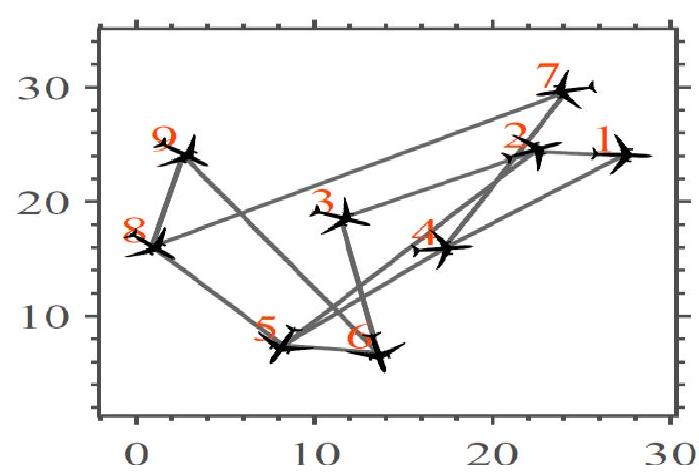
\includegraphics[max width=\textwidth]{2023_10_07_53b70c7408bc8e139415g-36(3)}
\end{center}

(a)

\begin{center}
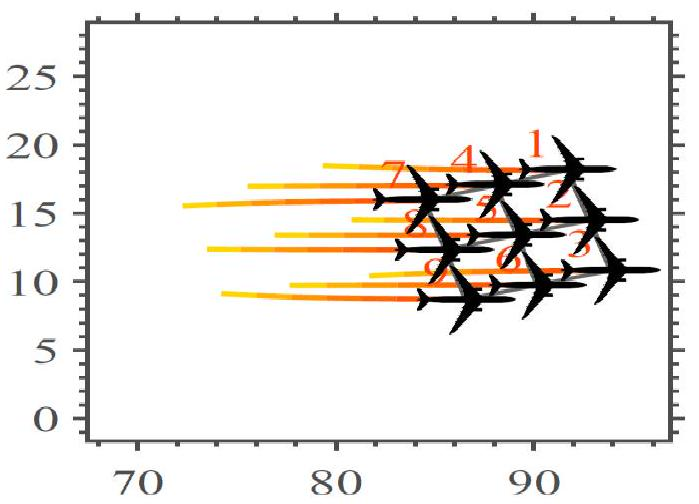
\includegraphics[max width=\textwidth]{2023_10_07_53b70c7408bc8e139415g-36(2)}
\end{center}

(c)

\begin{center}
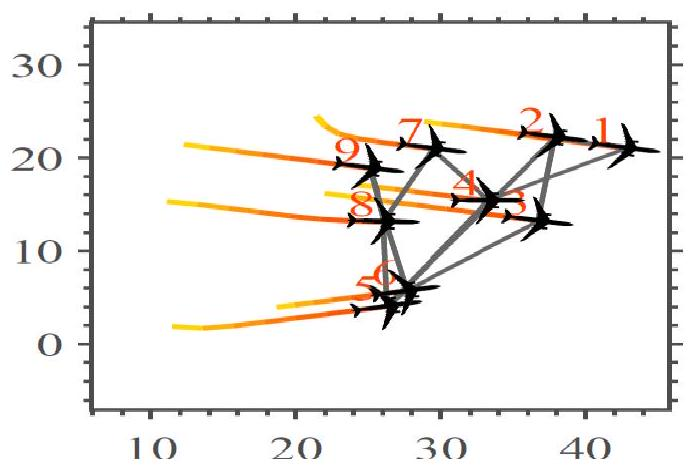
\includegraphics[max width=\textwidth]{2023_10_07_53b70c7408bc8e139415g-36}
\end{center}

(b)

\begin{center}
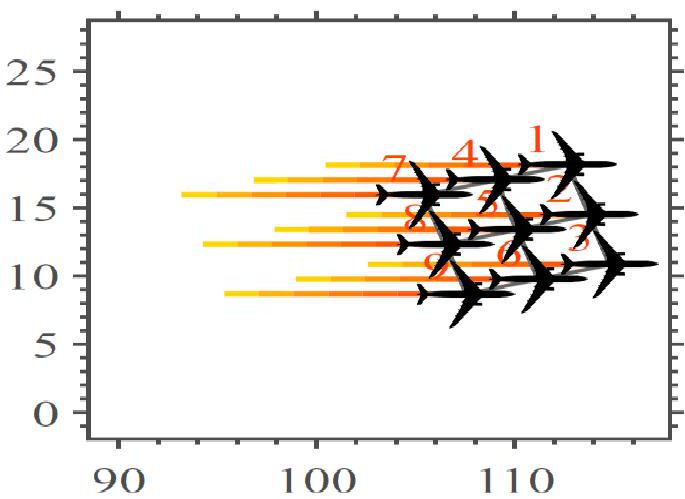
\includegraphics[max width=\textwidth]{2023_10_07_53b70c7408bc8e139415g-36(1)}
\end{center}

(d)

Fig 2.1: Simulation of 9 UAVs starting from a random initial pose and achieving a square formation while traveling along toward the positive $x$-axis. (a)Initial pose at (a)t $=0 \mathrm{~s}$. (b) $t=52 \mathrm{~s}$. (c) $\mathrm{t}=100 \mathrm{~s}$. (d) $\mathrm{t}=192 \mathrm{~s}$.

\begin{center}
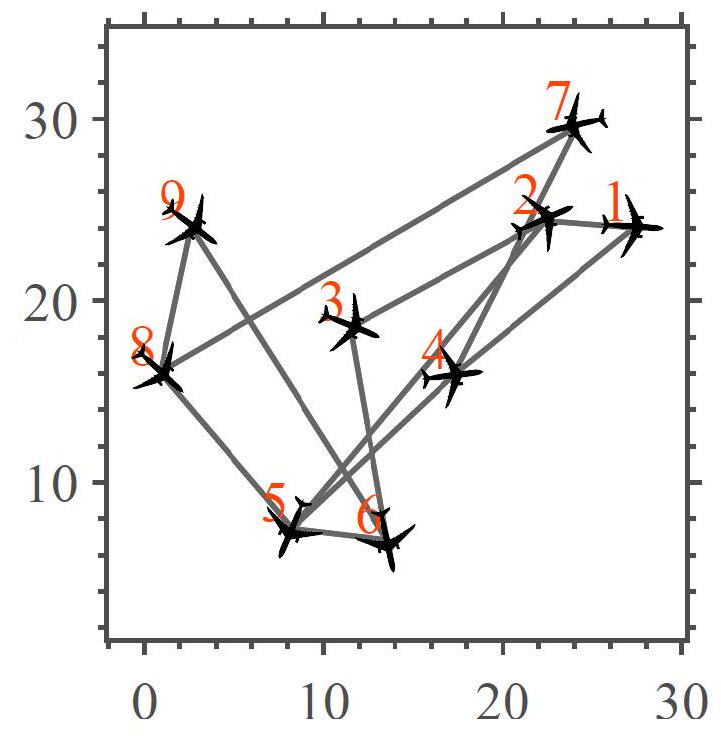
\includegraphics[max width=\textwidth]{2023_10_07_53b70c7408bc8e139415g-37(1)}
\end{center}

(a)

\begin{center}
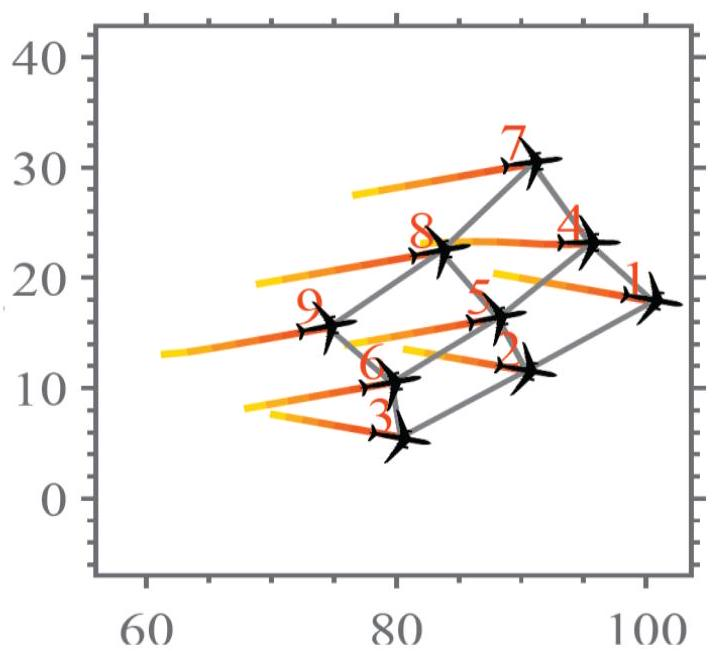
\includegraphics[max width=\textwidth]{2023_10_07_53b70c7408bc8e139415g-37}
\end{center}

(c)

\begin{center}
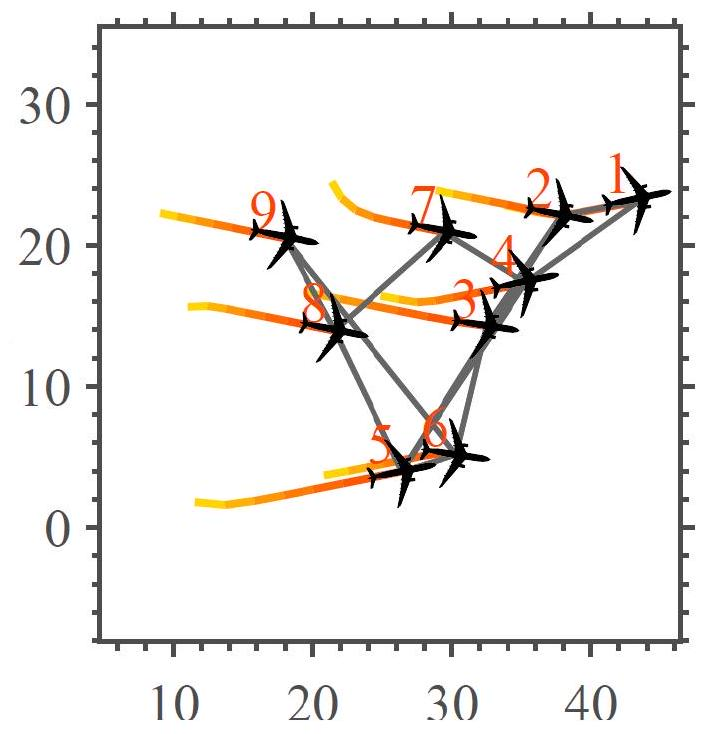
\includegraphics[max width=\textwidth]{2023_10_07_53b70c7408bc8e139415g-37(2)}
\end{center}

(b)

\begin{center}
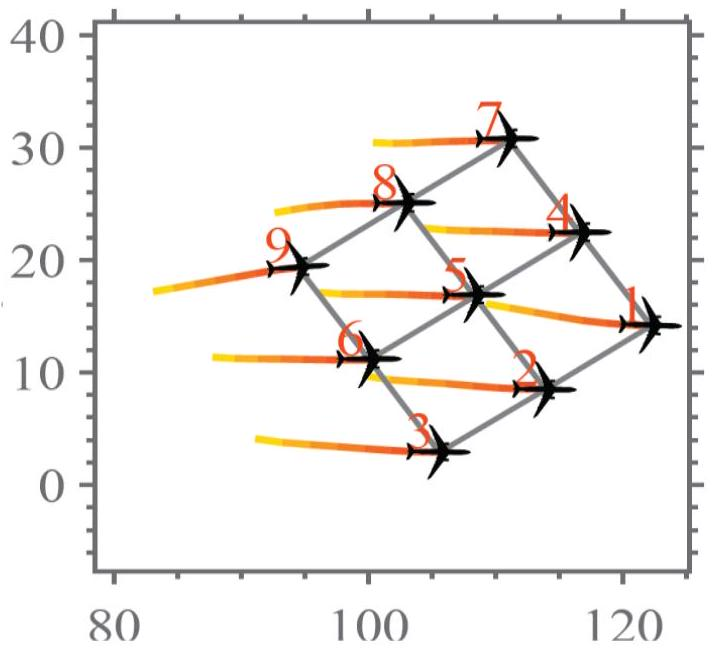
\includegraphics[max width=\textwidth]{2023_10_07_53b70c7408bc8e139415g-37(3)}
\end{center}

(d)

Fig 2.2: Simulation of 9 UAVs starting from a random initial pose and achieving a square formation with fixed scale while traveling along toward the positive $\mathrm{x}$-axis. (a)Initial pose at (a)t= 0s. (b) $t=52 s$. (c) $t=100 s$. (d) $t=192 s$.

\subsubsection{Triangle Formation}
\begin{center}
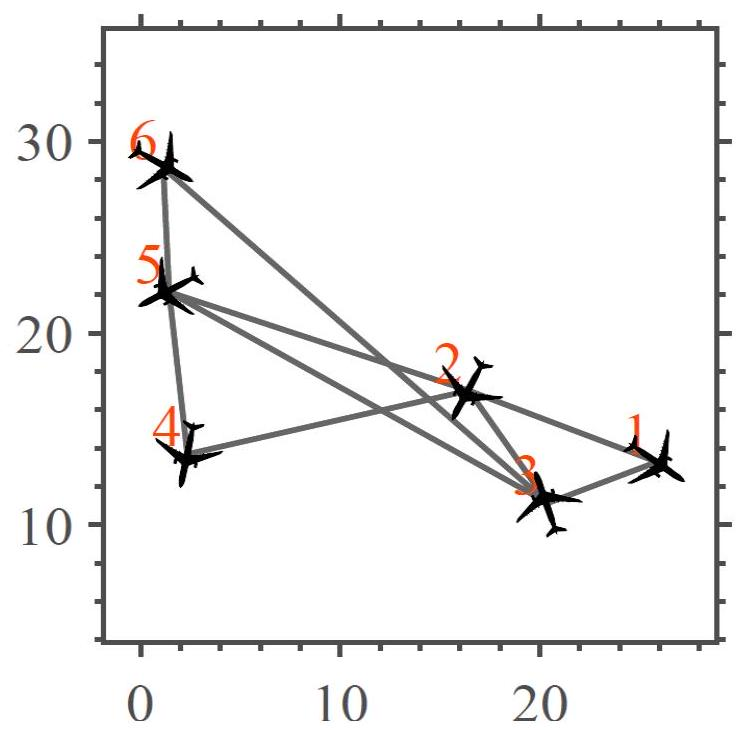
\includegraphics[max width=\textwidth]{2023_10_07_53b70c7408bc8e139415g-38(2)}
\end{center}

(a)

\begin{center}
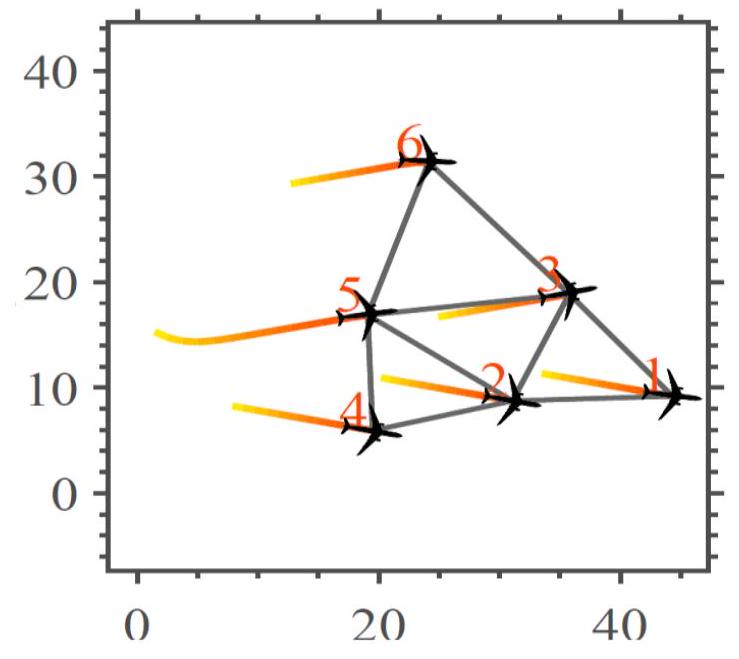
\includegraphics[max width=\textwidth]{2023_10_07_53b70c7408bc8e139415g-38(1)}
\end{center}

(c)

\begin{center}
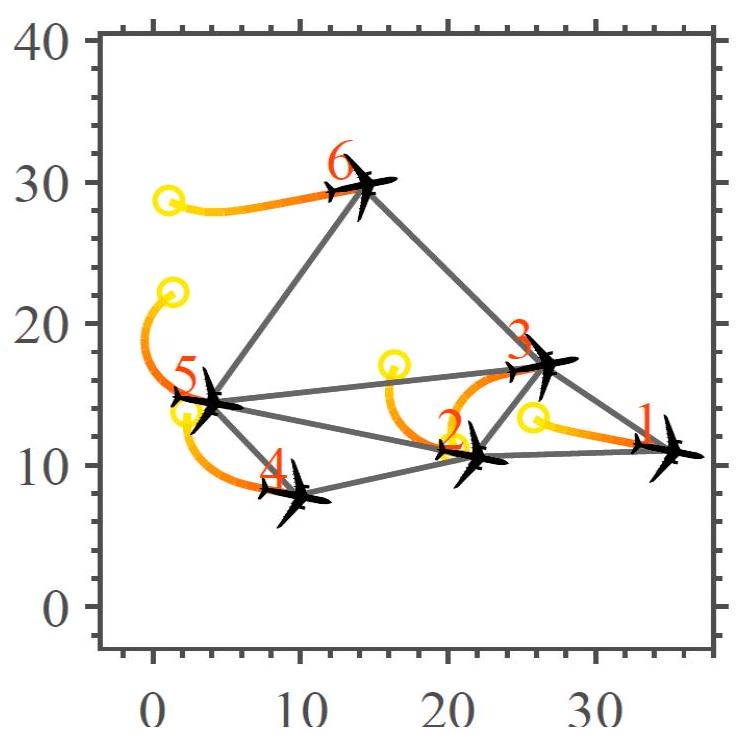
\includegraphics[max width=\textwidth]{2023_10_07_53b70c7408bc8e139415g-38(3)}
\end{center}

(b)

\begin{center}
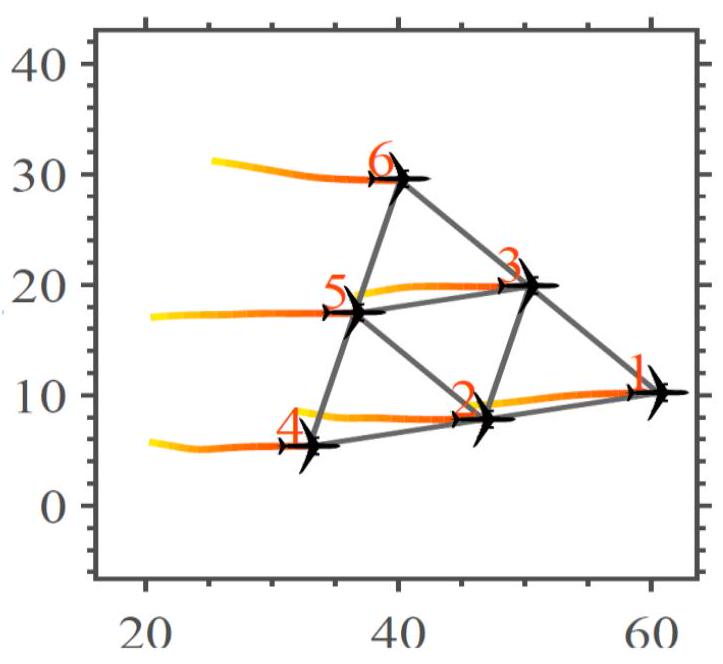
\includegraphics[max width=\textwidth]{2023_10_07_53b70c7408bc8e139415g-38}
\end{center}

(d)

Fig. 2.3: Simulation of 6 UAVs starting from a random initial pose and achieving a triangle formation while traveling along toward the positive $x$-axis. Initial pose at (a) $t=0$ s. (b) $t=31$ s. (c) $t=63 s$. (d) $t=102 \mathrm{~s}$.

\begin{center}
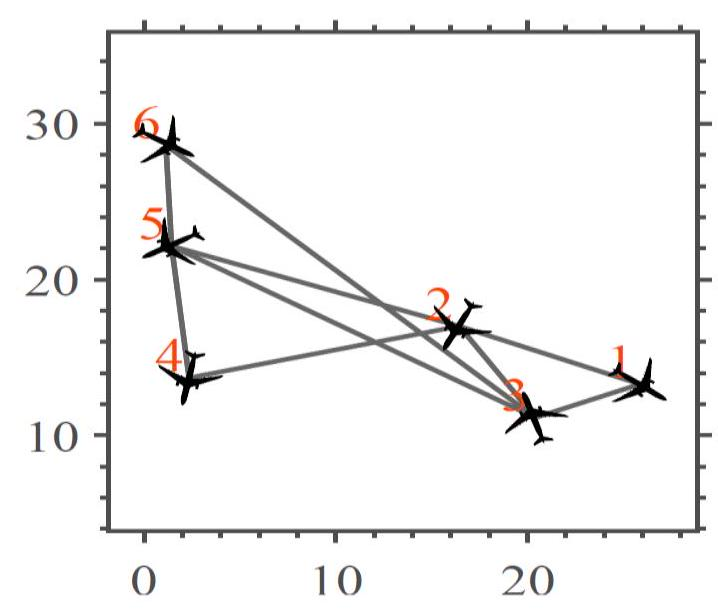
\includegraphics[max width=\textwidth]{2023_10_07_53b70c7408bc8e139415g-39(3)}
\end{center}

(a)

\begin{center}
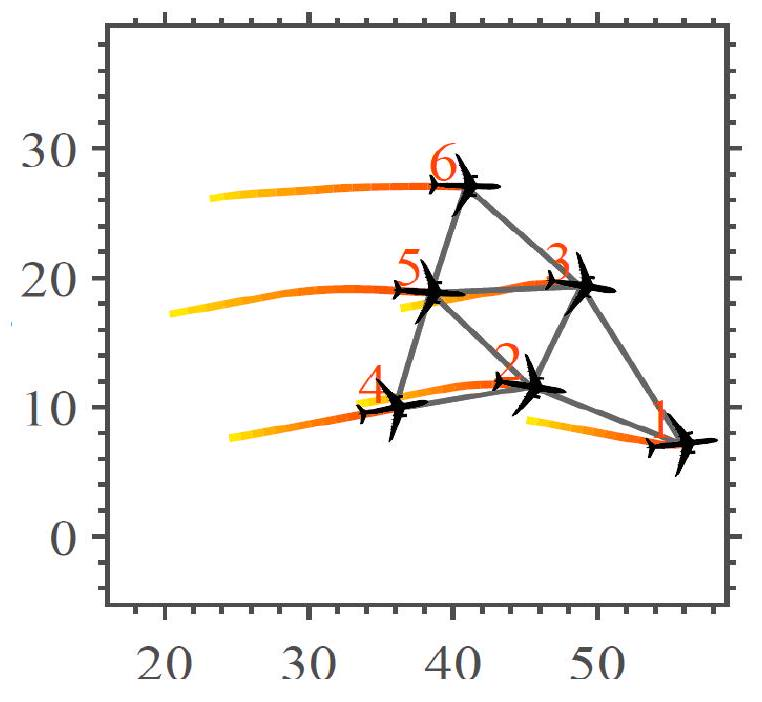
\includegraphics[max width=\textwidth]{2023_10_07_53b70c7408bc8e139415g-39(2)}
\end{center}

(c)

\begin{center}
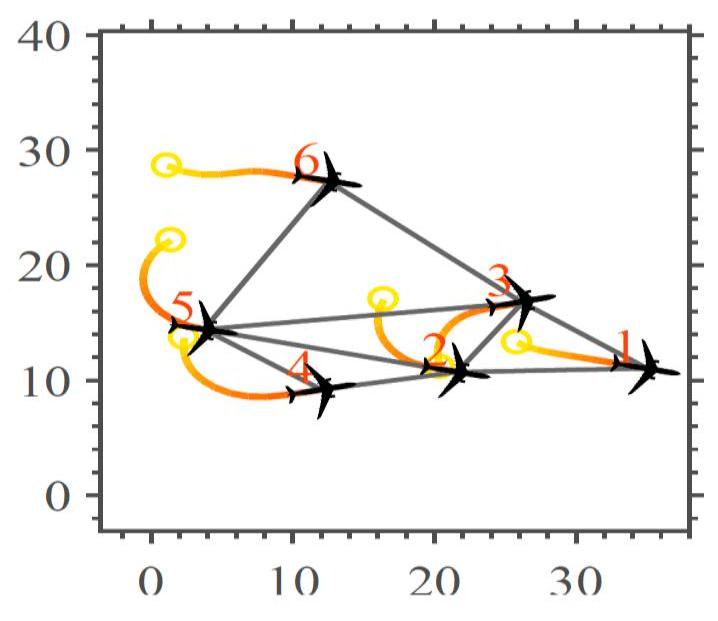
\includegraphics[max width=\textwidth]{2023_10_07_53b70c7408bc8e139415g-39(1)}
\end{center}

(b)

\begin{center}
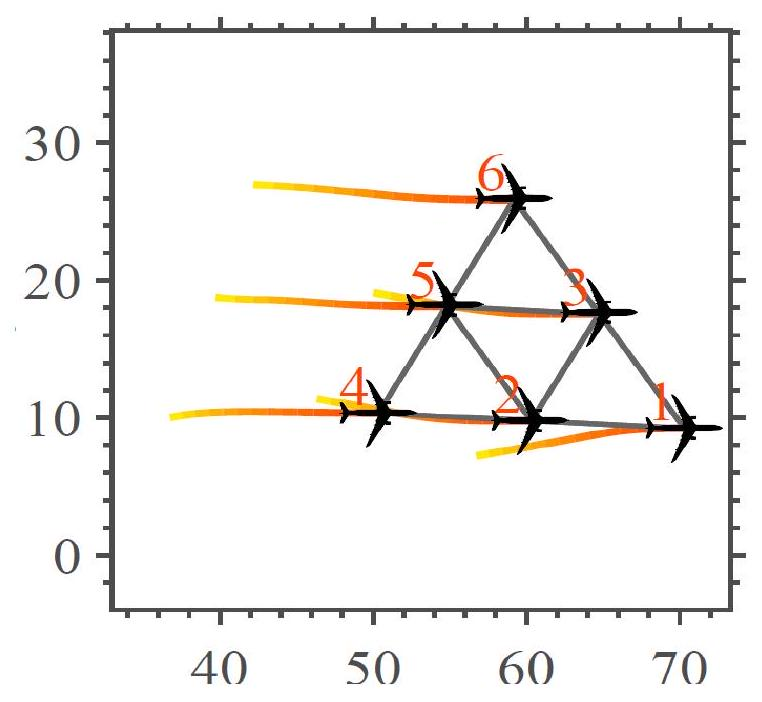
\includegraphics[max width=\textwidth]{2023_10_07_53b70c7408bc8e139415g-39}
\end{center}

(d)

Fig 2.4: Simulation of 6 UAVs starting from a random initial pose and achieving a triangle formation while traveling along toward the positive $x$-axis. Initial pose at (a)t $=0 \mathrm{~s}$. (b) $t=31$ s. (c) $\mathrm{t}=63 \mathrm{~s}$. (d) $\mathrm{t}=102 \mathrm{~s}$.

\subsection{Concluding Remarks and Future Work}
We presented a distributed formation control strategy for a team of UAVs to autonomously achieve and maintain a desired formation while traveling toward a desired destination. Given a desired formation, we showed how stabilizing control gains can be found from solving a convex optimization problem. These gains, which can be communicated to the agents before start of the mission, were used to calculate linear and angular velocity control commands for the UAVs under the Dubins constraint. Simulations were provided to show that under the proposed control the UAVs achieve the desired formation and travel along the assigned direction. Proof of convergence for the saturated UAV control is a topic of future work. To preserve connectivity, avoid obstacles, or prevent collision among UAVs, distributed techniques such as potential field traffic circle or control barrier function approach can be employed. Another strategy is a temporary change of altitude, i.e., UAVs passing over or under each other to avoid collision. This strategy can preserve the stability properties, however, the low-level altitude controller can become more complicated. Incorporating collision/obstacle avoidance strategies with the proposed formation control and analyzing the stability properties of the resulting system will be a topic of future work.Lastly, we assumed that the inter-agent sensing topology is fixed through all time. Strategies such as can be deployed when the sensing topology is time-varying or switching.

\section{CHAPTER III}
\section{PLANAR FORMATION CONTROL FOR HIGHER-ORDER HOLONOMIC AND NONHOLONOMIC AGENTS}
In this Chapter, we present a unified control strategy for agents with linear (or linearizable) holonomic dynamics. This strategy is distributed, only local relative position measurements are needed, and convergence to the desired formation is global. These advantages distinguish our approach from many existing works, such as the position-based or displacementbased methods (K.K. Oh et al. 2015), in which know ledge of a global coordinate frame or a common sense of orientation is required. By formulating a semidefinite programming (SDP) problem, formation control gains are initially designed for agents with the single-integrator model. We show that this design enjoys a robustness property, where if the agents move in the desired direction perturbed by a rotation up to $\pm 90^{\circ}$, convergence to the desired formation is still guaranteed. Furthermore, the control can be augmented by an integrator term to reject constant input/output disturbances. Our analysis follows by considering agents with higher order holonomic dynamics, where we show how the set of previously designed control gains can be used directly to achieve the formation. As an example, we use the proposed method for a team of quadrotors and present simulations to typify the theoretical results. In this work, we present a unified distributed control strategy for planar formations of agents with a variety of dynamics. In particular, we consider agents with linear or linearizable holonomic dynamics, such as quadrotors, and further extend the control to agents with nonholonomic dynamics such as unicycles and cars. We start by formulating a semidefinite programming (SDP) problem to determine control gains for agents with the single-integrator model. We show that this design strategy enjoys several robustness properties such as robustness to saturations in the input, switching in the sensing topology, and disturbances in the control direction. We show that if agents move along a control direction that is scaled by an arbitrary positive value and rotated by an arbitrary amount up to $\pm 90^{\circ}$, corvergence to the desired formation is still guaranteed. This observation is exploited later to design a fully distributed collision avoidance strategy. The control for single-integrator agents is extended subsequently to agents with higher-order holonomic dynamics, where we show the set of control gains computed from the SDP problem can be used directly to achieve the formation without having to redesign the control. As an example, we use the gains designed for single-integrator agents to achieve a planar formation of quadrotors. Following the same philosophy, we show that the control gains can be used directly for agents with nonholonomic dynamics such as unicycles and cars. Furthermore, the proposed nonholonomic control remains robust to input saturations and unmodeled/unknown dynamics. To vet the theoretical results, several simulations are presented for quadrotors, differential drive robots with unicycle dynamics, and cars, where it is shown that agents achieve a desired formation without collision. To simplify the results further, the proposed control strategy is tested experimentally on a distributed differential-drive wheeled robotic platform with different numbers of robots and desired formations.

\subsection{Notation and Assumptions}
We consider a team of $n \in \mathbb{N}$ agents with the inter-agent sensing topology described by an undirected graph $\mathcal{S}=(\mathcal{V}, \mathcal{E})$, where $\mathcal{V}:=\mathbb{N}_{n}$ is the set of vertices, and $\varepsilon \subset v \times v$ is the set of edges. Each vertex of the graph represents an agent. An edge from vertex $i \in \mathcal{V}$ to $j \in \mathcal{V}$ indicates that agents $i$ and $j$ can measure the relative position of each other in their local coordinate frames. In such a case, agents $i$ and $j$ are called neighbors. The set of neighbors of agent $i$ is denoted by $\mathcal{N}_{i}:=\{j \in \mathcal{V} \mid(i, j) \in \mathcal{E}\}$. We denote by eig $(A) \subset \mathbb{C}$ the set of eigenvalues of matrix $A$. Throughout this paper we assume that the desired formation and the sensing topology are such that achieving the formation is physically feasible. In particular, we assume that the sensing topology is undirected and universally rigid. This assumption is both necessary and sufficient (Z. Lin et al.2016), for guaranteeing the existence of control gains that are computed from the proposed SDP approach. We further point out that by "formation" we imply a desired geometric shape up to a positive scale factor.

\subsection{Problem statement}
In the distributed formation control literature, Agents often have, more complicated dynamics which makes control to agents with higher-order models is difficult. It lessens stability of the desired formation. Due to noise, disturbances, unmodeled dynamics, etc., often agents do not perfectly move along the desired control direction. Because of this Steady state errors induced by the friction. As a result, the convergence to the desired formation is affected for which collision between agents can happen. We present a distributed formation control strategy for agents with a variety of dynamics to achieve a desired planar formation. The proposed strategy is fully distributed, does not require inter-agent communication or a common sense of Orientation. We show how the control designed for agents with the simplest dynamical model, i.e., the single-integrator dynamics, can be extended to holonomic agents with higher-order dynamics such as quadrotors, and nonholonomic agents such as unicycles.

We further show that the control is relaxed in the sense that agents can move along a rotated and scaled control direction without affecting the convergence to the desired formation. This observation is used to design a distributed collision avoidance strategy.

\subsection{Robustness to Perturbations}
An important characteristic of the proposed design approach is that the gains found via (3.10) lead to significant robustness to perturbations. For instance, noise and disturbances can cause an agent to move in a direction that is different from the desired control vector. The following theorem shows that by using the gains computed from (3.10) positive scaling and rotation of the control vectors (up to $\pm 90^{\circ}$ ) does not affect the convergence.

Theorem 2. let $R_{i} \in \mathrm{SO}(2)$ denote a rotation matrix of $\alpha_{i}$ radians, and $c_{i} \in \mathbb{R}$ be a scalar. If $\alpha_{i} \in$ $\left(-\frac{\pi}{2}, \frac{\pi}{2}\right)$ and $c_{i}>0$, under the perturbed control

$$
u_{i}:=c_{i} R_{i} \sum_{j \in \mathcal{N}_{i}} A_{i j}\left(q_{j}-q_{i}\right)
$$

single-integrator agents achieve the desired formation.

Proof. We will use Definition 1 and Lemmas 2,3,4 that are given in the Appendix. Under the perturbed control (3.1), the aggregate dynamics can be represented by $\grave{q}=R A q$, where $R:=$ $\operatorname{diag}\left(c_{1} R_{1}, c_{2} R_{2}, \ldots, c_{n} R_{n}\right) \in \mathbb{R}^{2 n \times 2 n}$ is a block diagonal matrix that contains the perturbation terms. Due to the special block structure of $A$ and $R$, they can equivalently be represented in complex notation by denoting the $2 \times 2$ blocks $\left[\begin{array}{cc}a & -b \\ b & a\end{array}\right]$ as a complex number $a+\imath b \in \mathbb{C}$. In this notation, diagonal entries of $R \in \mathbb{C}^{n \times n}$ are $\cos \left(\alpha_{i}\right)+\imath \sin \left(\alpha_{i}\right)$,and since $\alpha_{i} \in\left(-\frac{\pi}{2}, \frac{\pi}{2}\right)$, have positive real parts. This, together with Lemma 3, implies that $\mathcal{F}(R)$ is contained in the right-hand plane (RHP). By design, the complex representation of $A \in \mathbb{C}^{n \times n}$ is Hermitian and negative semidefinite. Thus, $-A$ is positive semidefinite, and from Lemma 4 we conclude that eig $(-R A)$ is contained in the union of the RHP and the imaginary axis. Thus, $R A$ is a stable matrix, and trajectories of $\grave{q}=R A q$ converge to the kernel of $R A$. Since $R$ is full-rank, null space of $A$ and $R A$ are identical, which shows that the desired formation is achieved.

\subsection{Formation Control for Agents with Higher-Order Dynamics}
In this section, we extend the single-integrator control strategy to agents with higherorder dynamics. We show how the control gains designed for single-integrator agents in Section 3.2.2 can be used directly to control higher-order agents without having to find a new control strategy or redesign the gains by solving a new optimization problem. We assume that the aggregate higher-order dynamics of all agents can be expressed in the controllable canonical form

$$
\left[\begin{array}{c}
\grave{q} \\
\grave{q}^{(1)} \\
\vdots \\
\grave{q}^{(m-1)} \\
\grave{q}^{(m)}
\end{array}\right]=\left[\begin{array}{ccccc}
0 & I & 0 & \cdots & 0 \\
0 & 0 & I & & 0 \\
\vdots & & & \ddots & \vdots \\
0 & 0 & 0 & & I \\
0 & 0 & 0 & \cdots & 0
\end{array}\right]\left[\begin{array}{c}
q \\
q^{(1)} \\
\vdots \\
q^{(m-1)} \\
q^{(m)}
\end{array}\right]+\left[\begin{array}{c}
0 \\
0 \\
\vdots \\
0 \\
I
\end{array}\right] u
$$

where $q \in \mathbb{R}^{2 n}$ is the aggregate position vector of all agents, $q^{(j)} \in \mathbb{R}^{2 n}$ denotes the $j$ 'th derivative of $q$, and $I \in \mathbb{R}^{n \times n}$ is the identity matrix. Although at first sight (3.2) may seem restrictive, in fact, it encompasses a large class of agents. This is because by coordinate transformation techniques such as feedback linearization, or approximation techniques such as linearization and gain scheduling, dynamics of many systems can be expressed as (3.2). Given the gain matrix $A$ designed for agents with the singleintegrator model, the control for agents with dynamics (18) can be chosen as

$$
u=k_{0} A q+k_{1} A q^{(1)}+\cdots+k_{m} A q^{(m)}
$$

where $k_{0}, k_{1}, \ldots, k_{m} \in \mathbb{R}$ are scalar control gains.(3.3) can be implemented locally using only the relative measurements (due to the special structure of $A$ ). Under this control, the closed-loop dynamics is given by

$$
\left[\begin{array}{c}
\grave{q} \\
\grave{q}^{(1)} \\
\vdots \\
\grave{q}^{(m-1)} \\
\grave{q}^{(m)}
\end{array}\right]=\underbrace{\left[\begin{array}{ccccc}
0 & I & 0 & \cdots & 0 \\
0 & 0 & I & & 0 \\
\vdots & & & \ddots & \vdots \\
0 & 0 & 0 & & I \\
k_{0} A & k_{1} A & k_{2} A & \cdots & k_{m} A
\end{array}\right]}_{\breve{A}}\left[\begin{array}{c}
q \\
q^{(1)} \\
\vdots \\
q^{(m-1)} \\
q^{(m)}
\end{array}\right] .
$$

Theorem 4. If for all nonzero $\mu \in$ eig $(A)$ roots of the polynomial equation

$$
\lambda^{m+1}-k_{m} \mu \lambda^{m}-\cdots-k_{1} \mu \lambda-k_{0} \mu=0
$$

have negative real parts, then under control (3.3), agents with dynamics (3.2) globally converge to the desired formation.

Proof. The closed-loop state matrix $\bar{A}$ given in (3.4) is in the (block) controllable canonical form. From this observation and Lemma 5 (found in the Appendix), the characteristic equation of $\bar{A}$ is given by

$$
\begin{aligned}
& \operatorname{det}\left(\lambda^{m+1} I-k_{m} \lambda^{m} A-\cdots-k_{1} \lambda A-k_{0} A\right) \\
& =\prod_{\mu \in \operatorname{eig}(A)}\left(\lambda^{m+1} I-k_{m} \lambda^{m} \mu-\cdots-k_{1} \lambda \mu-k_{0} \mu\right)=0
\end{aligned}
$$

which from the assumption of the theorem implies that the nonzero eigenvalues of $\bar{A}$ have negative real parts.

To find gains $k_{0}, k_{1}, \ldots, k_{m}$ that satisfy the condition of Theorem 4 the Routh-Hurwitz criterion can be used.

Example 2. (Quadrotor dynamics) Quadrotor dynamics can be described as (F. Sabatino, 2015)

$$
\begin{aligned}
{\left[\begin{array}{l}
\grave{x} \\
\grave{y} \\
\grave{z}
\end{array}\right]=R\left[\begin{array}{l}
0 \\
0 \\
u^{a}
\end{array}\right]-\left[\begin{array}{l}
0 \\
0 \\
g
\end{array}\right] } \\
{\left[\begin{array}{l}
\grave{\varphi} \\
\grave{\theta} \\
\grave{\psi}
\end{array}\right]=T\left[\begin{array}{l}
\omega_{x} \\
\omega_{y} \\
\omega_{z}
\end{array}\right] } \\
{\left[\begin{array}{l}
\hat{\omega}_{x} \\
\grave{\omega}_{y} \\
\hat{\omega}_{z}
\end{array}\right]=J^{-1}\left[\begin{array}{l}
u^{x} \\
u^{y} \\
u^{z}
\end{array}\right]-J^{-1}\left(\left[\begin{array}{c}
\omega_{x} \\
\omega_{y} \\
\omega_{z}
\end{array}\right] \times J\left[\begin{array}{c}
\omega_{x} \\
\omega_{y} \\
\omega_{z}
\end{array}\right]\right) }
\end{aligned}
$$

where, $x, y, z \in \mathbb{R}$ are coordinates of the quadrotor's center of mass in the world frame, $\varphi, \theta, \psi$ are roll, pitch, yaw angles that describe the orientation of the quadrotor body frame in the world frame, $\omega_{x}, \omega_{y}, \omega_{z}$ are the angular body rates about associated body axes, $g$ is the gravitational constant, $u^{a}$ is a mass-normalized thrust input, and $u^{x}, u^{y}, u^{z}$ are moment inputs applied to the airframe about corresponding body axes. Further, $J \in \mathbb{R}^{3 \times 3}$ is the mass moment of inertia matrix, $R \in \mathrm{SO}(3)$ is the rotation matrix parameterized in terms of $z-x-y$ Euler angles as

$$
R:=\left[\begin{array}{ccc}
c_{\psi} c_{\theta}-s_{\varphi} s_{\psi} s_{\theta} & -c_{\varphi} s_{\psi} & c_{\psi} s_{\theta}+c_{\theta} s_{\varphi} s_{\psi} \\
c_{\theta} s_{\psi}+c_{\psi} s_{\varphi} s_{\theta} & c_{\varphi} c_{\psi} & s_{\psi} s_{\theta}-c_{\psi} c_{\theta} s_{\varphi} \\
-c_{\varphi} s_{\theta} & s_{\varphi} & c_{\varphi} c_{\theta}
\end{array}\right]
$$

where $c, s$ are respectively shorthand notations for $\cos (\cdot), \sin (\cdot)$ functions, and

$$
T:=\frac{1}{c_{\varphi}}\left[\begin{array}{ccc}
c_{\varphi} c_{\theta} & 0 & -c_{\theta} \\
s_{\varphi} s_{\theta} & c_{\varphi} & -c_{\theta} s_{\varphi} \\
-s_{\theta} & 0 & c_{\theta}
\end{array}\right] \in \mathbb{R}^{3 \times 3}
$$

is the transformation matrix that relates the roll, pitch, yaw derivatives to the angular velocities in the body frame. Linearizing dynamics about the hover point $x=y=z=\grave{x}=\grave{y}=\grave{z}=$ $0, \omega_{x}=\omega_{y}=\omega_{z}=0, u^{x}=u^{y}=u^{z}=0$, and $u^{a}=g$ gives the quadrotor linearized dynamics,

$$
\begin{array}{ll}
\delta \grave{x}=g \delta \theta & \delta \grave{\theta}=u^{y} \\
\delta \grave{y}=-g \delta \varphi & \delta \grave{\varphi}=u^{x} \\
\delta \grave{z}=u^{a} & \delta \grave{\psi}=u^{z}
\end{array}
$$

where $\delta$ represents a small displacement about the equilibrium/linearization point. Since we are interested in 2D formations, we only consider the lateral dynamics along the $x-y$ axes, and separately control the quadrotor's altitude by setting $u^{a}=\frac{g}{c_{\varphi} c_{\theta}}$ to stabilize it at a constant altitude.

To represent the dynamics in the canonical form (3.4), we define

$$
\delta \grave{\theta}_{i}:=g \delta \theta_{i}, \delta \overleftarrow{\varphi}_{i}:=-g \delta \varphi_{i}, \bar{u}_{i}^{y}:=g u_{i}^{y}, \bar{u}_{i}^{x}:=-g u_{i}^{x}
$$

where subscript $i$ is used to distinguish agents. Using this notation, (3.10) can be described in the vector form as

$$
\grave{p}_{i}=\left[\begin{array}{cccc}
0 & I & 0 & 0 \\
0 & 0 & I & 0 \\
0 & 0 & 0 & I \\
0 & 0 & 0 & 0
\end{array}\right] p_{i}+\left[\begin{array}{l}
0 \\
0 \\
0 \\
I
\end{array}\right] u_{i}
$$

Where

$$
\begin{aligned}
& p_{i}:=\left[\delta x_{i}, \delta y_{i}, \delta \grave{x}_{i}, \delta \grave{y}_{i}, \delta \bar{\theta}_{i}, \delta \bar{\varphi}_{i}, \delta \grave{\bar{\theta}}_{i}, \delta \grave{\bar{\varphi}}_{i}\right]^{\top} \\
& u_{i}:=\left[\bar{u}_{i}^{y}, \bar{u}_{i}^{x}\right]^{\top}
\end{aligned}
$$

are respectively the state and control vectors, and $I \in \mathbb{R}^{2 \times 2}$ is the identity matrix. Note that by

defining the aggregate position vector as $q=\left[\delta x_{1}, \delta y_{1}, \ldots, \delta x_{n}, \delta y_{n}\right]^{\top}$, dynamics of agents can be expressed in the form (3.4). This model will be used in the Simulations section to achieve a desired formation.

\subsection{Simulations}
To validate the proposed approach, several simulations for planar formation of quadrotors, unicycles are provided.

\subsubsection{Quadrotors}
Fig. 9(a) - (d) shows the top view of quadrotors at different time instances. The sensing graph among agents is shown by gray lines connecting the quadrotors. The initial positions of the quadrotors are chosen randomly and are shown in Fig. 9(a). As can be seen in Figs. 9( b) - (d), the proposed control strategy brings the agents to the desired formation. Note that when the distance between two quadrotors becomes less than 8 units of length, the collision avoidance strategy is engaged to rotate the control direction outside of the collision cone. Consequently, none of the quadrotors collide during the simulation. Further notice that since the control only uses the local relative position measurements, the desired formation is achieved up to a rotation and translation. That is, the orientation of the square formation is not controlled.

\begin{center}
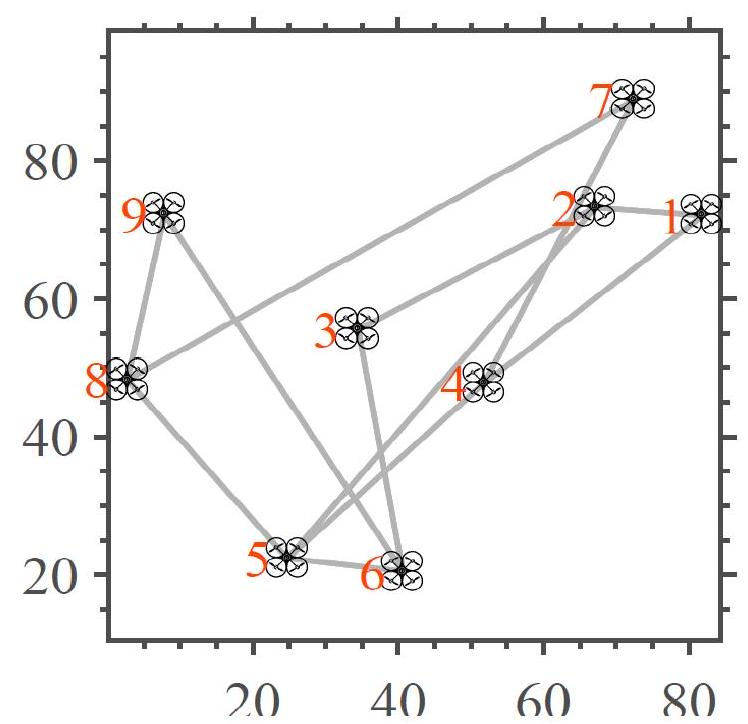
\includegraphics[max width=\textwidth]{2023_10_07_53b70c7408bc8e139415g-50(1)}
\end{center}

(a)

\begin{center}
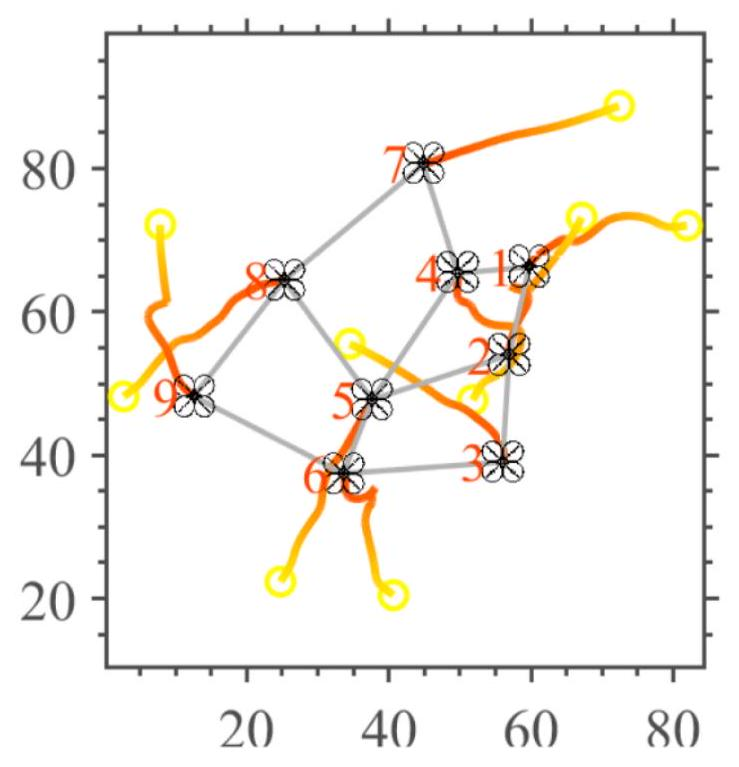
\includegraphics[max width=\textwidth]{2023_10_07_53b70c7408bc8e139415g-50}
\end{center}

(c)

\begin{center}
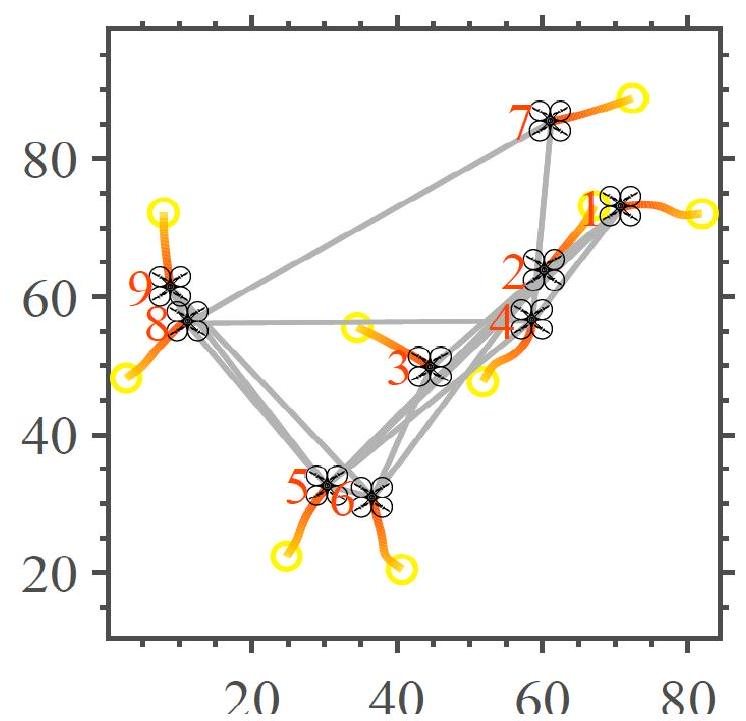
\includegraphics[max width=\textwidth]{2023_10_07_53b70c7408bc8e139415g-50(3)}
\end{center}

(b)

\begin{center}
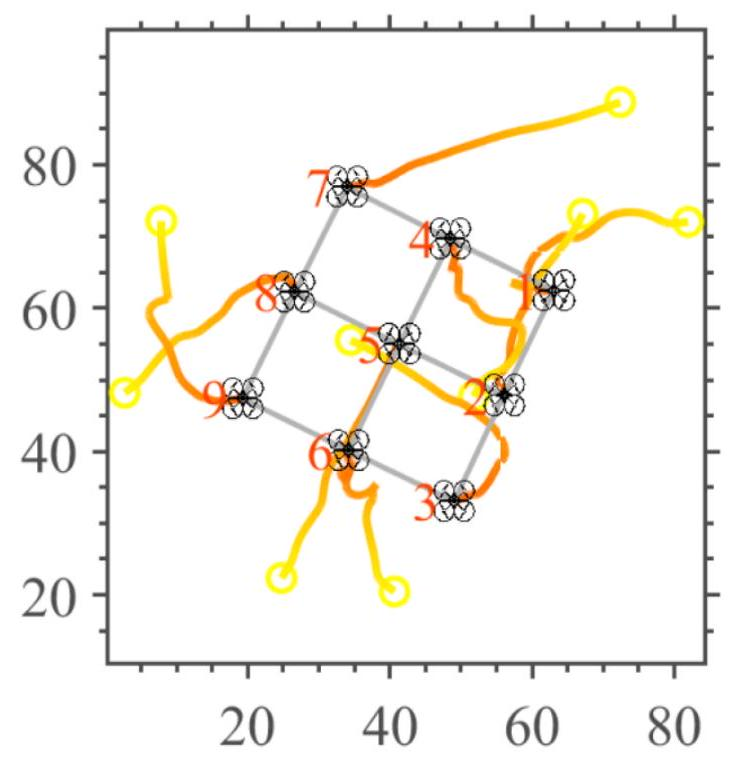
\includegraphics[max width=\textwidth]{2023_10_07_53b70c7408bc8e139415g-50(2)}
\end{center}

(d)

Fig. 3.1. Simulation of 9 quadrotors with a square grid desired formation (actual size of vehicles increased by a factor of 1.5 for better visibility). (a) Top view at $t=0 \mathrm{~s}$. (b) $t=17 \mathrm{~s}$. (c) $t=29 \mathrm{~s}$. (d) $\mathrm{t}=40 \mathrm{~s}$.

\begin{center}
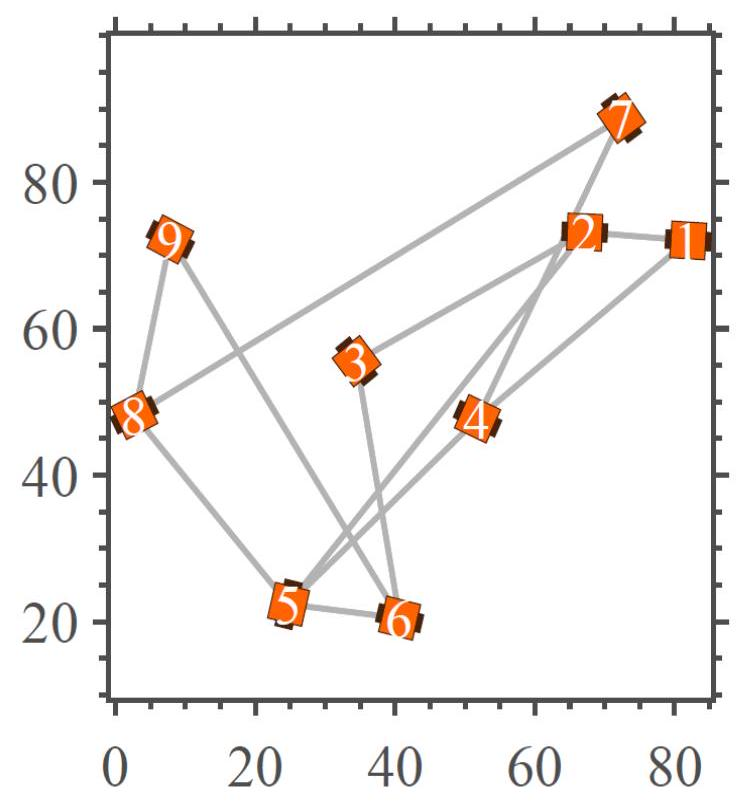
\includegraphics[max width=\textwidth]{2023_10_07_53b70c7408bc8e139415g-51(1)}
\end{center}

(a)

\begin{center}
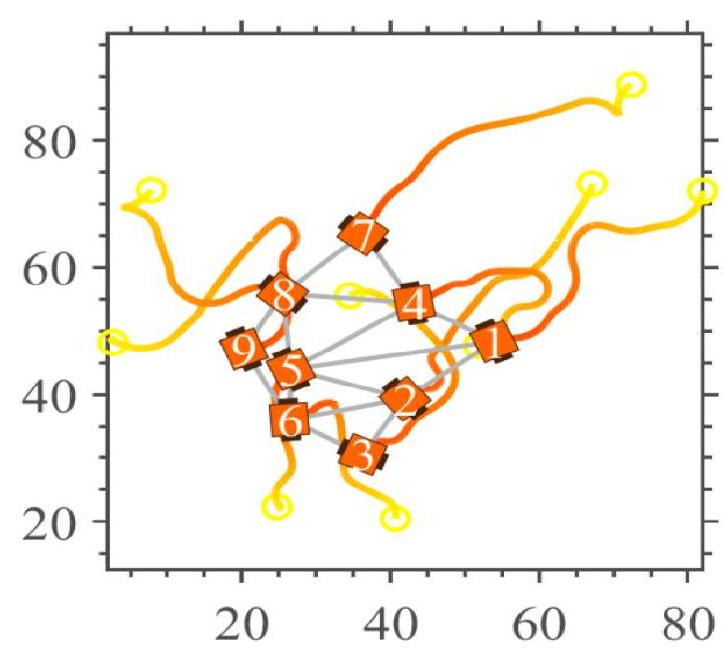
\includegraphics[max width=\textwidth]{2023_10_07_53b70c7408bc8e139415g-51}
\end{center}

(c)

\begin{center}
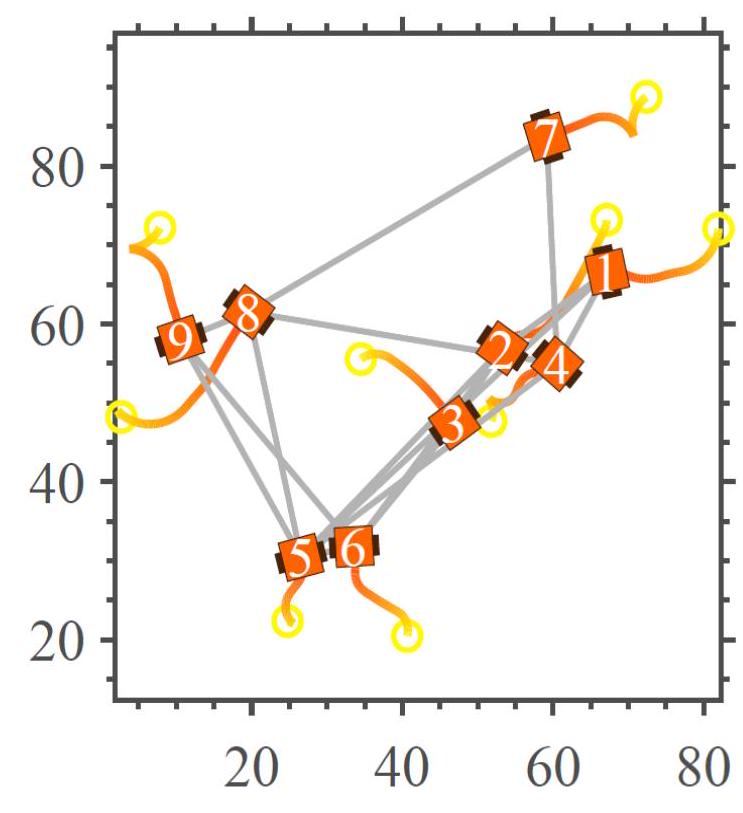
\includegraphics[max width=\textwidth]{2023_10_07_53b70c7408bc8e139415g-51(3)}
\end{center}

(b)

\begin{center}
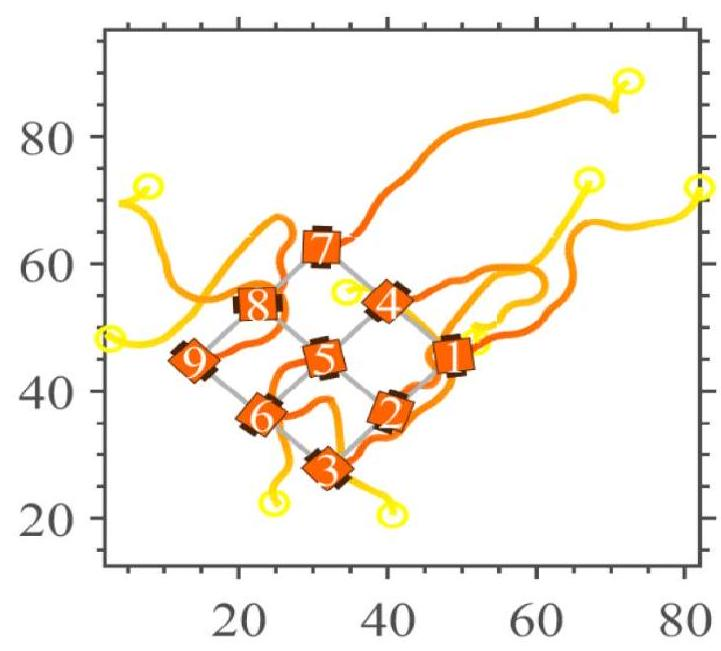
\includegraphics[max width=\textwidth]{2023_10_07_53b70c7408bc8e139415g-51(2)}
\end{center}

(d)

Fig. 3.2 Simulation of 9 unicycles with a square grid desired formation (actual size of vehicles increased by a factor of 1.5 for better visibility). (a) Top view at $t=0$ s. (b) $t=6 s$. (c) $t=9 s$. (d) $t$ $=15 \mathrm{~s}$.

\subsection{Concluding Remarks and Future Work}
We presented a distributed formation control strategy for a team of agents with a variety of dynamics to autonomously achieve a desired planar formation. Under the assumption that the sensing graph is undirected and universally rigid, we showed that formation control gains can be designed by solving a SDP problem. This design enjoys several robustness properties, such as robustness to positive scaling and rotation (( up to $\left.\pm 90^{\circ}\right)$ of the control vector, saturations in the input, and switches in the sensing topology. The control was extended to agents with higherorder linear (or linearizable) holonomic dynamics, such as quadrotors, followed by further extension to agents with nonholonomic unicycle and car dynamics. An important outcome of this work was a fully distributed collision avoidance algorithm that emerged naturally from the robustness properties of the proposed strategy. To typify the control, simulations for vehicles with different dynamics were presented, and experiments on a distributed robotic platform where performed. Future work includes investigating additional requirements, such as inter-agent communication, to guarantee that the collision avoidance algorithm can overcome gridlock scenarios. Moreover, inter-agent communication can be exploited in a distributed optimization scheme to solve the SDP problem in decentralized way. Other possible research avenues include extending the proposed approach to 3D formations, formation control of heterogeneous vehicles, and formation control of moving vehicles such as cars on a highway.

\section*{CHAPTER IV }
\section{DISTRIBUTED COMMAND FILTERED ROBUST TRACKING CONTROL OF WAVE-ADAPTIVE MODULAR VESSEL WITH UNCERTAINTY}


\subsection{Problem Statement}
\subsubsection{WAM-V Modeling}
It is considered a group of m wave-adaptive modular vessels (WAM-Vs). Each WAMV

has two propellers in its pontoons. With the aid of the results in (Fossen, 1994), the kinematics of the $\mathrm{j}$-th WAM-V can be written as

$$
\begin{aligned}
\grave{x}_{j} & =u_{j} \cos \psi_{j}-v_{j} \sin \psi_{j} \\
\grave{y}_{j} & =u_{j} \sin \psi_{j}+v_{j} \cos \psi_{j} \\
\grave{\psi}_{j} & =r_{j}
\end{aligned}
$$

where $\left(x_{j}, y_{j}\right)$ denotes the coordinates of the center of the WAM-V in the earth-fixed frame, $\psi_{j}$ is the orientation of the WAM-V, and $u_{j}, v_{j}$ and $r_{j}$ are the velocities of the WAM-V in surge, sway and yaw, respectively. For simplicity of analysis, it is assumed that the $j$ th WAM-V has port/starboard and fore/aft symmetry and the motion in heave, roll and pitch can be neglected. The dynamics of the $j$ th WAM-V can be written as (Fossen, 1994)

$$
\begin{gathered}
m_{1 j} \grave{u}_{j}-m_{2 j} v_{j} r_{j}+d_{1 j} u_{j}+D_{1 j}=F_{L j}+F_{R j} \\
m_{2 j} \grave{v}_{j}+m_{1 j} u_{j} r_{j}+d_{2 j} v_{j}+D_{2 j}=0 \\
m_{3 j} \grave{r}_{j}-\left(m_{1 j}-m_{2 j}\right) u_{j} v_{j}+d_{3 j} r_{j}+D_{3 j}=L_{j}\left(F_{L j}-F_{R j}\right)
\end{gathered}
$$

where $m_{i j}(>0)$ and $d_{i j}(>0)$ for $i=1,2,3$ are (effective) inertia and hydrodynamic damping of the WAM-V, respectively; $L_{j}$ is the moment arm of the forces with respect to the center of geometry and mass of the WAM-V, which are assumed to coincide; $D_{i j}$ is un-modeled dynamics and disturbance, and $F_{L j}$ and $F_{R j}$ are the force generated by the propellers. For control purpose, each WAM-V knows its own state and the states of its neighbors by wireless communication or sensors. If each WAM-V is considered as a node, the communications between WAM-Vs can be described by a directed graph (i.e., digraph) $\mathcal{G}=$ $\{\mathcal{V}, \mathcal{E}\}$, where $\mathcal{V}=\{1,2, \ldots, m\}$ is a node set, $\mathcal{E}$ is an edge set with elements $(i, j)$ which describes the communication from node $i$ to node $j$. If the state of node $i$ is available to node $j$, there is an edge $(i, j)$ in $\mathcal{E}$, and vice versa. Node $i$ is a neighbor of node $j$ if the state of node $i$ is available to node $j$. Since communication is directional, $(i, j)$ is an ordered pair, which means that $(i, j) \in \mathcal{E}$ does not mean $(j, i) \in \mathcal{E}$. For node $j$, the indexes of its neighbors form a set which is denoted by $\mathcal{N}_{j}$. Therefore, the available states to node $j$ are the state of node $j$ and the state of node $i$ for all $i \in \mathcal{N}_{j}$. A directed path in a digraph is an ordered sequence of vertices such that any ordered pair of vertices appearing consecutively in the sequence is an edge of the digraph. Node $i$ is reachable to node $j(j \neq i)$ if there exists a directed path from node $i$ to node $j$.

\subsubsection{Problem Statement}
In the dynamics (4)-(6), the inertia parameters $m_{i j}$ and $d_{i j}$ are not exactly known in practice. It is given a leader WAM-V which moves along a smooth trajectory $\left(x_{0}(t), y_{0}(t)\right)$. The leader WAM-V is labeled as node 0 . The $m$ WAM-Vs in (1)-(3) are called the follower WAMVs. The state of the leader WAM-V is available to some of the follower WAM-Vs. The communication between $m$ follower WAM-Vs and the leader WAM-V is described by a digraph $\mathcal{G}^{e}=\left\{\mathcal{V}^{e}, \mathcal{E}^{e}\right\}$ with a node set $\mathcal{V}^{e}=0,1,2, \ldots, m$. For node $j(0 \leq j \leq m)$, its neighbor set is denoted as $\mathcal{N}_{j}^{e}$. Node 0 is said to be globally reachable if node 0 is reachable to node $j$ for $1 \leq$ $j \leq m$. In this paper, the following assumption is made on the communication digraph $\mathcal{G}^{e}$

Assumption 1: In the communication digraph $\mathcal{G}^{e}$, node 0 is globally \href{http://reachable.It}{reachable.It} is also given a desired geometric pattern $\mathcal{P}$ defined by constant vectors $\left[p_{j x}, p_{j y}\right]^{\top}(1 \leq j \leq m)$ which satisfy $\sum_{j=1}^{m} p_{j x}=0$ and $\sum_{j=1}^{m} p_{j y}=0$. We consider the following formation control problem.

Formation Control Problem: Design a controller $\left(F_{L j}, F_{R j}\right)$ for $j$-th follower WAM-V based on its neighbors' state information such that

$$
\begin{aligned}
& \lim _{t \rightarrow \infty}\left[\begin{array}{l}
x_{i}-x_{j} \\
y_{i}-y_{j}
\end{array}\right]=\left[\begin{array}{l}
p_{i x}-p_{j x} \\
p_{i y}-p_{j y}
\end{array}\right], 1 \leq i, j \leq m \\
& \lim _{t \rightarrow \infty} \sum_{j=1}^{m}\left(\frac{x_{j}}{m}-x_{0}\right)=0 \\
& \lim _{t \rightarrow \infty} \sum_{j=1}^{m}\left(\frac{y_{j}}{m}-y_{0}\right)=0
\end{aligned}
$$

In the above problem, eqn. (4.3) means that $m$ follower WAM-Vs come into the desired geometric pattern $\mathcal{P}$.

\subsection{Distributed Robust Controller Design}
It is assumed that the nominal values of $m_{i j}$ and $d_{i j}$ are $\bar{m}_{i j}$ and $\bar{d}_{i j}$, respectively. The errors between the nominal values and the real values are bounded by known constants, i.e., $\left|m_{1 j}-\bar{m}_{1 j}\right| \leq \rho_{1 j},\left|m_{2 j}-\bar{m}_{2 j}\right| \leq \rho_{2 j},\left|m_{3 j}-\bar{m}_{3 j}\right| \leq$ $\rho_{3 j},\left|d_{1 j}-\bar{d}_{1 j}\right| \leq \rho_{4 j},\left|d_{3 j}-\bar{d}_{3 j}\right| \leq \rho_{5 j},\left|D_{1 j}\right| \leq \rho_{6 j}$, and $\left|D_{3 j}\right| \leq \rho_{7 j}$, where $\rho_{i j}(1 \leq i \leq 7)$ are known. The system in (4.1) -(4.2) has a cascade structure. We will take this advantage and design a distributed controller for the $j$-th WAM-V with the aid of backstepping techniques (Krstic et al., 1995).

Step 1: For system $j$, the weighted average of its neighbor's information is defined as

$$
\zeta_{1 j}=\frac{\sum_{i \in \mathcal{N}_{j}^{e}} a_{j i}\left(x_{i}-p_{i x}\right)}{\sum_{i \in \mathcal{N}_{j}^{e}} a_{j i}}, \zeta_{2 j}=\frac{\sum_{i \in \mathcal{N}_{j}^{e}} a_{j i}\left(y_{i}-p_{i y}\right)}{\sum_{i \in \mathcal{N}_{j}^{e}} a_{j i}}
$$

where $\mathcal{N}_{j}^{e}$ is the neighbor set of node $j$ in the $\operatorname{digraph} \mathcal{G}^{e}, a_{j i}$ is a positive constant for $j=$ $1,2, \ldots, m$. In the system (4.1)-(4.2), we consider $u_{j} \cos \psi_{j}$ and $u_{j} \sin \psi_{j}$ as virtual control inputs and design tracking controllers such that

$$
\begin{aligned}
& \lim _{t \rightarrow \infty}\left(x_{j}(t)-p_{j x}-\zeta_{1 j}(t)\right)=0 \\
& \lim _{t \rightarrow \infty}\left(y_{j}(t)-p_{j y}-\zeta_{2 j}(t)\right)=0
\end{aligned}
$$

For convenience, we let

$$
u_{j} \cos \psi_{j}=\eta_{1 j}, u_{j} \sin \psi_{j}=\eta_{2 j}
$$

where $\eta_{1 j}$ and $\eta_{2 j}$ will be chosen later. Let the tracking error

$$
e_{* j}=\left[\begin{array}{l}
e_{1 j} \\
e_{2 j}
\end{array}\right]=\left[\begin{array}{l}
x_{j}-p_{j x}-\zeta_{1 j} \\
y_{j}-p_{j y}-\zeta_{2 j}
\end{array}\right]
$$

then

$$
\grave{e}_{* j}=\left[\begin{array}{l}
\eta_{1 j} \\
\eta_{2 j}
\end{array}\right]+\left[\begin{array}{c}
-\sin \psi_{j} \\
\cos \psi_{j}
\end{array}\right] v_{j}-\left[\begin{array}{c}
\grave{\zeta}_{1 j} \\
\grave{\zeta}_{2 j}
\end{array}\right]
$$

(4.8) can be considered as a linear system with perturbations. Stabilizing controllers can be designed as

$$
\begin{aligned}
& \eta_{1 j}=-a_{j j} e_{1 j}+v_{j} \sin \psi_{j}-\frac{\rho_{x} e_{1 j}}{\sqrt{e_{1 j}^{2}+h(t)}} \\
& T_{2 j}=-a_{j j} e_{2 j}-v_{j} \cos \psi_{j}-\frac{\rho_{y} e_{2 j}}{\sqrt{e_{2 j}^{2}+h(t)}}
\end{aligned}
$$

where $a_{j j}=\sum_{i \in \mathcal{N}}=a_{j i}, \rho_{x}$ and $\rho_{y}$ are sufficiently large constants, $h(t)>0$, and $h(t)$ exponentially converges to zero.

To verify that the proposed virtual controller (4.9) ensures that (4.5)hold, we substitute the virtual controller (4.9) to (4.1) - (4.2) and have

$$
\begin{aligned}
& \grave{x}_{j}=-\sum_{i \in \mathcal{N}_{j}^{\prime}} a_{j i}\left(x_{j}-p_{j x}-x_{i}+p_{i x}\right)-\frac{\rho_{x} e_{1 j}}{\sqrt{e_{i j}^{2}+h}} \\
& \grave{y}_{j}=-\sum_{i \in N_{j}^{\prime}} a_{j i}\left(y_{j}-p_{j y}-y_{i}+p_{i y}\right)-\frac{\rho_{y} e_{2 j}}{\sqrt{e_{2 j}^{2}+h}}
\end{aligned}
$$

Define $\bar{x}_{j}=x_{j}-p_{j x}-x_{0}$ and $\vec{y}_{j}=y_{j}-p_{j y}-y_{0}$ where

$p_{0 x}=p_{0 y}=0$, we have

$$
\begin{aligned}
& \grave{\grave{x}}_{j}=-\sum_{i \in N_{j}^{*}} a_{j i}\left(\bar{x}_{j}-\bar{x}_{i}\right)-\grave{x}_{0}-\frac{\rho_{x} e_{1 j}}{\sqrt{e_{1 j}^{2}+h}} \\
& \overline{\bar{y}}_{j}=-\sum_{i \in \mathcal{N}_{j}^{*}} a_{j i}\left(\bar{y}_{j}-\grave{y}_{i}\right)-\grave{y}_{0}-\frac{\rho_{y} e_{2 j}}{\sqrt{e_{2 j}^{2}+h}}
\end{aligned}
$$

For the communication between vehicles we make the following assumption.

Assumption 2: The leader vehicle is globally reachable. If

$$
\rho_{x} \geq \mathrm{m}\left\{\left|\grave{x}_{0}(t)\right|\right\}, \rho_{y} \geq \mathrm{m}\left\{\left|\grave{y}_{0}(t)\right|\right\}
$$

it can be proved that $\bar{x}_{j}$ and $\bar{y}_{j}$ exponentially converge to zero if Assumption 2 is satisfied with the aid of the results in [Dong, 2013]

By (4.6), we solve $u_{j}$ and $\psi_{j}$ and obtain $u_{j}=T_{3 j}$ and $\psi_{j}=\eta_{4 j}$ where

$$
T_{3 j}=\sqrt{\eta_{1 j}^{2}+\eta_{2 j}^{2}}, \eta_{4 j}=\operatorname{atan} 2\left(T_{2 j}, \eta_{1 j}\right)
$$

In (4.12), atan 2 is not defined if $\eta_{2 j}=0$ and $T_{1 j}=0$. To avoid this, we make the following assumption. Assumprion 3: $0<\epsilon<\grave{x}_{0}^{2}(t)+\grave{y}_{0}^{2}(t)<\infty$ for any time $t$, where $\epsilon$ is a small positive constant Step 2: $u_{j}$ and $\psi_{j}$ are not the real control inputs and $\left[u_{j}, \psi_{j}\right]^{\top} \neq$ $\left[T_{j j}, \eta_{4 j}\right]^{T}$. Let

$$
z_{v j}=\left[z_{1 j}, s_{2 j}\right]^{\top}=\left[u_{j}-\eta_{\beta j}, \psi_{j}-\eta_{H j}\right]^{\top}
$$

then

$$
\begin{aligned}
\grave{\dot{x}}_{j}= & -\sum_{i \in \mathcal{N}_{j}^{e}} a_{j i}\left(\grave{x}_{j}-\grave{x}_{i}\right)-\grave{x}_{0}-\frac{\rho_{x} e_{1 j}}{\sqrt{e_{1 j}^{2}+h}} \\
\grave{y}_{J}= & -\sum_{i \in \mathcal{N}_{j}^{e}} a_{j i}\left(\grave{y}_{j}-\grave{y}_{i}\right)-\grave{y}_{0}-\frac{\rho_{y} e_{2 j}}{\sqrt{e_{2 j}^{2}+h}} \\
& +\Omega_{j} \\
m_{1 j} \grave{z}_{1 j}= & m_{2 j} v_{j} r_{j}-d_{1 j} u_{j}+F_{L j}+F_{R j} \\
& -m_{1 j} \grave{\eta}_{3 j}-D_{1 j} \\
\grave{z}_{2 j}= & r_{j}-\grave{\eta}_{4 j}
\end{aligned}
$$

Where,

$$
\begin{aligned}
\Lambda_{j}= & z_{1 j} \cos \eta_{4 j}+u_{j} z_{2 j} \cos \eta_{4 j} \frac{\left(\cos z_{2 j}-1\right)}{z_{2 j}} \\
& -u_{j} z_{2 j} \sin \eta_{4 j} \frac{\sin z_{2 j}}{z_{2 j}} \\
\Omega_{j}= & z_{1 j} \sin \eta_{4 j}+u_{j} z_{2 j} \sin \eta_{4 j} \frac{\left(\cos z_{2 j}-1\right)}{z_{2 j}} \\
& +u_{j} z_{2 j} \cos \eta_{4 j} \frac{\sin z_{2 j}}{z_{2 j}}
\end{aligned}
$$

for $1 \leq j \leq m$. For the system in (4.13), the following input-to-state property can be shown. Lemma 1: For the systems in (4.13), Under Assumption 2

1 if $z_{1 j}$ and $z_{2 j}$ are bounded and converge to a small neighborhood of the origin with radius $r, \grave{x}_{j}$ and $\grave{y}_{j}$ are bounded and converge to a neighborhood of the origin whose radius can be made as small as possible by choosing $r$ very small.

2 if $z_{1 j}$ and $z_{2 j}$ are bounded and converge to zero, $\bar{x}_{j}$ and $\grave{y}_{j}$ are bounded and converge to zero.

3 if $z_{1 j}$ and $z_{2 j}$ exponentially converge to zero, $\grave{x}_{j}$ and $\grave{y}_{j}$ exponentially converge to zero. The proof of Lemma 1 is omitted due to space limit. Thanks to Lemma 1, we design controllers such that $z_{1 j}$ and $z_{2 j}$ are bounded and converge to zero. Choose a Lyapunov function candidate

$$
V_{2 j}=\frac{1}{2} \sum_{j=1}^{m}\left(m_{1 j} z_{1 j}^{2}+z_{2 j}^{2}\right)
$$

and differentiate $V_{2 j}$ along the solution of the systems in (4.13), we have

$$
\begin{aligned}
\grave{V}_{2 j}= & \sum_{j=1}^{m} z_{1 j}\left[m_{2 j} v_{j} r_{j}-d_{1 j} u_{j}+F_{L j}+F_{R j}\right. \\
& \left.-m_{1 j} \grave{\eta}_{3 j}-D_{1 j}\right]+\sum_{j=1}^{m} z_{2 j}\left(r_{j}-\grave{\eta}_{4 j}\right)
\end{aligned}
$$

We choose

$$
\begin{aligned}
F_{L j}+F_{R j}= & -K_{3} z_{1 j}+\bar{m}_{1 j} \grave{\eta}_{3 j}-\bar{m}_{2 j} v_{j} r_{j}+\grave{d}_{1 j} u_{j} \\
& -\left(\rho_{1 j}\left|\grave{\eta}_{3 j}\right|+\rho_{2 j}\left|v_{j} r_{j}\right|\right. \\
& \left.+\rho_{4 j}\left|u_{j}\right|+\rho_{6 j}\right) \operatorname{sign}\left(z_{1 j}\right)=: \delta_{1 j} \\
r_{j}= & \eta_{5 j} \\
\eta_{5 j}= & -K_{4} z_{2 j}+\grave{\eta}_{4 j}
\end{aligned}
$$

where $K_{3}$ and $K_{4}$ are positive definite matrices. Then

$$
\grave{V}_{2 j} \leq-\sum_{j=1}^{m}\left(K_{3} z_{1 j}^{2}+K_{4} z_{2 j}^{2}\right)
$$

It can be shown that $z_{1 j}$ and $z_{2 j}(1 \leq j \leq m)$ are bounded and exponentially converge to zero.

\begin{itemize}
  \item Step 3: $r_{j}$ is not the real control inputs and $r_{j} \neq \eta_{5 j}$.
\end{itemize}

$$
\begin{aligned}
& \text { Let } z_{3 j}=r_{j}-\eta_{5 j} \text {, then } \\
& \grave{z}_{2 j}=-K_{4} z_{2 j}+z_{3 j} \\
& m_{3 j} \grave{z}_{3 j}=\left(m_{1 j}-m_{2 j}\right) u_{j} v_{j}-d_{3 j} r_{j}-m_{3 j} \grave{\eta}_{5 j} \\
& -D_{3 j}+L_{j}\left(F_{R j}-F_{L j}\right)
\end{aligned}
$$

Choose a Lyapunov function candidate

$$
V_{3 j}=V_{2 j}+\frac{1}{2} \sum_{j=1}^{m} m_{3 j} z_{3 j}^{2}
$$

and differentiate it along the solutions of the system, we have

$$
\begin{aligned}
\grave{V}_{3 j} \leq & -\sum_{j=1}^{m}\left(K_{3} z_{1 j}^{2}+K_{4} z_{2 j}^{2}\right)+\sum_{j=1}^{m} z_{2 j} z_{3 j} \\
& +\sum_{j=1}^{m} z_{3 j}\left(\left(m_{1 j}-m_{2 j}\right) u_{j} v_{j}-d_{3 j} r_{j}-m_{3 j} \grave{\eta}_{j j}\right. \\
& \left.-D_{3 j}+L_{j}\left(F_{R j}-F_{L j}\right)\right)
\end{aligned}
$$

We choose

$$
\begin{aligned}
L_{j}\left(F_{R j}-F_{L j}\right)= & -K_{5} z_{3 j}-z_{2 j}-\left(\bar{m}_{1 j}-\bar{m}_{2 j}\right) u_{j} v_{j} \\
& +\bar{d}_{3 j} r+\bar{m}_{3 j} \grave{\eta}_{5 j}-\left(\left(\rho_{1 j}\right.\right. \\
& \left.+\rho_{2 j}\right)\left|u_{j} v_{j}\right|+\rho_{5 j}\left|r_{j}\right|+\rho_{3 j}\left|\grave{\eta}_{5 j}\right| \\
& \left.+\rho_{7 j}\right) \operatorname{sign}\left(z_{3 j}\right)=: \delta_{2 j}
\end{aligned}
$$

where $K_{5}$ is a positive constant. Then

$$
\grave{V}_{3 j} \leq-\sum_{j=1}^{m}\left(K_{3} z_{1 j}^{2}+K_{4} z_{2 j}^{2}+K_{5} z_{3 j}^{2}\right)
$$

It can be shown that $z_{1 j}, z_{2 j}, z_{3 j}(1 \leq j \leq m)$ are bounded and exponentially converge to zero.

Solve the equations in (4.17) and (4.22), we obtain the control inputs as follows:

$$
F_{R j}=\frac{1}{2}\left(\delta_{1 j}+\frac{\delta_{2 j}}{L_{j}}\right), F_{L j}=\frac{1}{2}\left(\delta_{1 j}-\frac{\delta_{2 j}}{L_{j}}\right)
$$

The above results are summarized in the following theorem.

Theorem 1: For $m$ vehicles in (4.1-4.2)and a leader vehicle with the desired trajectory $\left(x_{0}, y_{0}\right)$, under Assumptions 1 - 3, the control laws in (4.24) ensure that (4.3) are satisfied.

\subsection{Distributed Command Filtered Tracking Control Laws}
In the proposed controller in the last section, the derivatives of signals are needed. To avoid this, a command filtered controller can be designed with the aid of the ideas in (Dong et al., 2012). To this end, we introduce the following command filters:

$$
\begin{aligned}
& \grave{\chi}_{1 j}=-r_{1 j}\left|\chi_{1 j}-\eta_{3 j}\right|^{\frac{1}{2}} \operatorname{sign}\left(\chi_{1 j}-\eta_{3 j}\right)+\chi_{2 j} \\
& \grave{\chi}_{2 j}=-r_{2 j} \operatorname{sign}\left(\chi_{2 j}-\grave{\chi}_{1 j}\right) \\
& \grave{\chi}_{3 j}=-r_{3 j}\left|\chi_{3 j}-\eta_{4 j}\right|^{\frac{1}{2}} \operatorname{sign}\left(\chi_{3 j}-\eta_{4 j}\right)+\chi_{4 j} \\
& \grave{\chi}_{4 j}=-r_{4 j} \operatorname{sign}\left(\chi_{4 j}-\grave{\chi}_{3 j}\right) \\
& \grave{\chi}_{5 j}=-r_{5 j}\left|\chi_{5 j}-\eta_{5 j}\right|^{\frac{1}{2}} \operatorname{sign}\left(\chi_{5 j}-\eta_{5 j}\right)+\chi_{6 j} \\
& \grave{\chi}_{6 j}=-r_{6 j} \operatorname{sign}\left(\chi_{6 j}-\grave{\chi}_{5 j}\right)
\end{aligned}
$$

The compensated signals are defined by

$$
\begin{array}{ll}
\dot{\xi}_{1 j} & =-\frac{K_{3}}{\bar{m}_{1 j}} \xi_{1 j} \\
\dot{\xi}_{2 j} & =-K_{4} \xi_{2 j}+\xi_{3 j}+\left(\chi_{5 j}-\eta_{5 j}\right) \\
\dot{\xi}_{3 j} & =-\frac{K_{5}}{\bar{m}_{3 j}} \xi_{3 j}
\end{array}
$$

Let

$$
\begin{aligned}
w_{1 j} & =u_{j}-\chi_{1 j}-\xi_{1 j} \\
w_{2 j} & =\psi_{j}-\chi_{3 j}-\xi_{2 j} \\
z_{3 j} & =r_{j}-\chi_{5 j}-\xi_{3 j}
\end{aligned}
$$

then

$$
\begin{aligned}
m_{1 j} \grave{w}_{1 j}= & m_{2 j} v_{j} r_{j}-d_{1 j} u_{j}+F_{L j}+F_{R j} \\
& -m_{1 j} \grave{\chi}_{1 j}-D_{1 j}-m_{1 j} \grave{\xi}_{1 j} \\
\grave{w}_{2 j}= & r_{j}-\grave{\chi}_{3 j}-\grave{\xi}_{2 j} \\
= & z_{3 j}+\bar{\xi}_{3 j}+\left(\chi_{5 j}-\eta_{5 j}\right)+\eta_{5 j} \\
& -\grave{\chi}_{3 j}-\grave{\xi}_{2 j} \\
m_{3 j} \grave{z}_{3 j}= & \left(m_{1 j}-m_{2 j}\right) u_{j} v_{j}-d_{3 j} r_{j}-m_{3 j} \grave{\chi}_{5 j} \\
& -D_{3 j}+L_{j}\left(F_{R j}-F_{L j}\right)-m_{3 j} \grave{\xi}_{3 j}
\end{aligned}
$$

We choose

$$
\begin{aligned}
F_{L j}+F_{R j}=\quad & -K_{3}\left(u_{j}-\chi_{1 j}\right)+\overleftarrow{m}_{1 j} \grave{\chi}_{1 j} \\
& -\bar{m}_{2 j} v_{j} r_{j}+\bar{d}_{1 j} u_{j}-\left(\rho_{1 j}\left|\grave{\chi}_{1 j}\right|\right. \\
& +\rho_{2 j}\left|v_{j} r_{j}\right|+\rho_{4 j}\left|u_{j}\right| \\
& \left.+\rho_{6 j}\right) \operatorname{sign}\left(w_{1 j}\right)=: \delta_{1 j} \\
L_{j}\left(F_{R j}-F_{L j}\right)=\quad & -K_{4} \psi_{j}+\grave{\chi}_{3 j} \\
\eta_{5}=\quad & -K_{5}\left(r_{j}-\chi_{s j}\right)-w_{2 j}-\left(\bar{m}_{1 j}\right. \\
& \left.-\bar{m}_{2 j}\right) u_{j} v_{j}+\bar{d}_{3 j} r+\bar{m}_{3 j} \grave{\chi}_{5 j} \\
& -\left(\left(\rho_{1 j}+\rho_{2 j}\right)\left|u_{j} v_{j}\right|+\rho_{5 j}\left|r_{j}\right|\right. \\
& \left.+\rho_{3 j}\left|\grave{\chi}_{5 j}\right|+\rho_{7 j}\right) \operatorname{sign}\left(z_{3 j}\right) \\
=: & \delta_{2 j}
\end{aligned}
$$

then (4.28) are in the following forms.

$$
\begin{aligned}
m_{1 j} \grave{w}_{1 j}= & -K_{3} w_{1 j}+\grave{m}_{2 j} v_{j} r_{j}-\grave{d}_{1 j} u_{j} \\
& -\grave{m}_{1 j} \grave{\chi}_{1 j}-D_{1 j}+\frac{m_{1 j}-\bar{m}_{1 j}}{\bar{m}_{1 j}} K_{3} \xi_{1 j} \\
& -\left(\rho_{1 j}\left|\grave{\chi}_{1 j}\right|+\rho_{2 j}\left|v_{j} r_{j}\right|\right. \\
& \left.+\rho_{4 j}\left|u_{j}\right|+\rho_{6 j}\right) \operatorname{sign}\left(w_{1 j}\right) \\
\grave{w}_{2 j}= & -K_{4} w_{2 j}+z_{3 j} \\
m_{3 j} \grave{z}_{3 j}= & \left(\grave{m}_{1 j}-\grave{m}_{2 j}\right) u_{j} v_{j}-\grave{d}_{3 j} r_{j}-\grave{m}_{3 j} \grave{\chi}_{5 j}-D_{3 j} \\
& -K_{5} z_{3 j}-w_{2 j}+\frac{m_{3 j}-\bar{m}_{3 j}}{\grave{m}_{3 j}} K_{5} \xi_{3 j} \\
& -\left(\left(\rho_{1 j}+\rho_{2 j}\right)\left|u_{j} v_{j}\right|+\rho_{5 j}\left|r_{j}\right|+\rho_{3 j}\left|\grave{\chi}_{s j}\right|\right. \\
& \left.+\rho_{7 j}\right) \operatorname{sign}\left(z_{3 j}\right)
\end{aligned}
$$

Theorem 2: For $m$ vehicles in (4.1)-(4.2) and a leader vehicle with the desired trajectory $\left(x_{0}, y_{0}\right)$, under Assumptions $1-3$, the control law in (4.24) with $\delta_{1 j}$ in (4.29) and $\delta_{2 j}$ in (4.30) ensure that (4.3) are satisfied.

Proof: Choose a Ly apunov function

$$
V_{4}=\frac{1}{2} \sum_{j=1}^{m}\left(m_{1 j} w_{1 j}^{2}+w_{2 j}^{2}+m_{3 j} z_{3 j}^{2}\right)
$$

its derivative along the solution of the closed loop system is

$$
\begin{aligned}
\grave{V}_{4} \leq \quad & -K_{3} w_{1 j}^{2}-K_{4} w_{2 j}^{2}-K_{5} z_{3 j}^{2} \\
& +\frac{m_{1 j}-\bar{m}_{1 j}}{\overleftarrow{m}_{1 j}} K_{3} \xi_{1 j} w_{1 j}+\frac{m_{3 j}-\bar{m}_{3 j}}{\overleftarrow{m}_{3 j}} K_{5} \xi_{3 j} z_{3 j}
\end{aligned}
$$

Noting that $\xi_{1 j}$ and $\xi_{3 j}$ exponentially converge to zero, it can be shown that $w_{1 j}, w_{2 j}$, and $z_{3 j}$ exponentially converge to zero, respectively. By the command filters, $\chi_{1 j}-\eta_{3 j}, \chi_{3 j}-\eta_{4 j}$, and $\chi_{5 j}-\eta_{5 j}$ are bounded and converge to zero in a finite time. By the definitions of the compensated signals, $\xi_{1 j}, \xi_{3 j}$, and $\xi_{2 j}$ exponentially converge to zero. So, $z_{1 j}$ and $z_{2 j}$ converge to zero. By Lemma $1, \grave{x}_{j}$ and $\grave{y}_{j}$ converge to zero, which means that (4.7) - (4.9) are satisfied.

\subsection{Simulation}
Consider three identical WAM-Vs with the model parameters: $m_{1 j}=200, m_{2 j}=$ $250, m_{3 j}=80, d_{1 j}=70, d_{2 j}=100, d_{3 j}=50$ for $j=1,2,3$. The un-modeled dynamics and uncertainty is as follows: $D_{1 j}=2 \cos 0.3 t, D_{2 j}=2 \cos 0.2 t$, and $D_{3 j}=2 \cos 0.1 t$. Assume the desired geometric pattern $\mathcal{P}$ is a triangle defined by $\left(p_{1 x}, p_{1 y}\right)(0,20),\left(p_{2 x}, p_{2 y}\right)=$ $(-20,-10)$, and $\left(p_{3 x}, p_{3 y}\right)=(20,-10)$. (see Fig. 1$)$. The desired trajectory $\left(x_{0}, y_{0}\right)=$ $(20 \cos 0.1 t, 20 \sin 0.1 t)$

Assume the communication digraph $\mathcal{G}$ among the WAMVs is fixed and is shown in Fig. 2. The communication graph is directed. If the estimates of inertia parameters are known as

$\overleftarrow{m}_{1 j}=210, \bar{m}_{2 j}=240, \overleftarrow{m}_{3 j}=75, \bar{d}_{1 j}=75, \bar{d}_{2 j}=105, \bar{d}_{3 j}=55$ for $j=1,2,3$. The bounds between the estimations can be chosen as $\rho_{1 j}=10, \rho_{2 j}=10, \rho_{3 j}=10, \rho_{4 j}=10, \rho_{\mathfrak{s} j}=$ $10, \rho_{6 j}=3$, and $\rho_{7 j}=4$. The cooperative control laws can be obtained by Theorem 2. Figs. $4-$ 4 show the time response of $\grave{x}_{j}$ and $\grave{y}_{j}$ for $1 \leq j \leq 3$. Figs. $5-7$ show the time response of $z_{1 j}, z_{2 j}$, and $z_{3 j}$ for $1 \leq j \leq 3$. The simulation results verify Theorem 1 .

\begin{center}
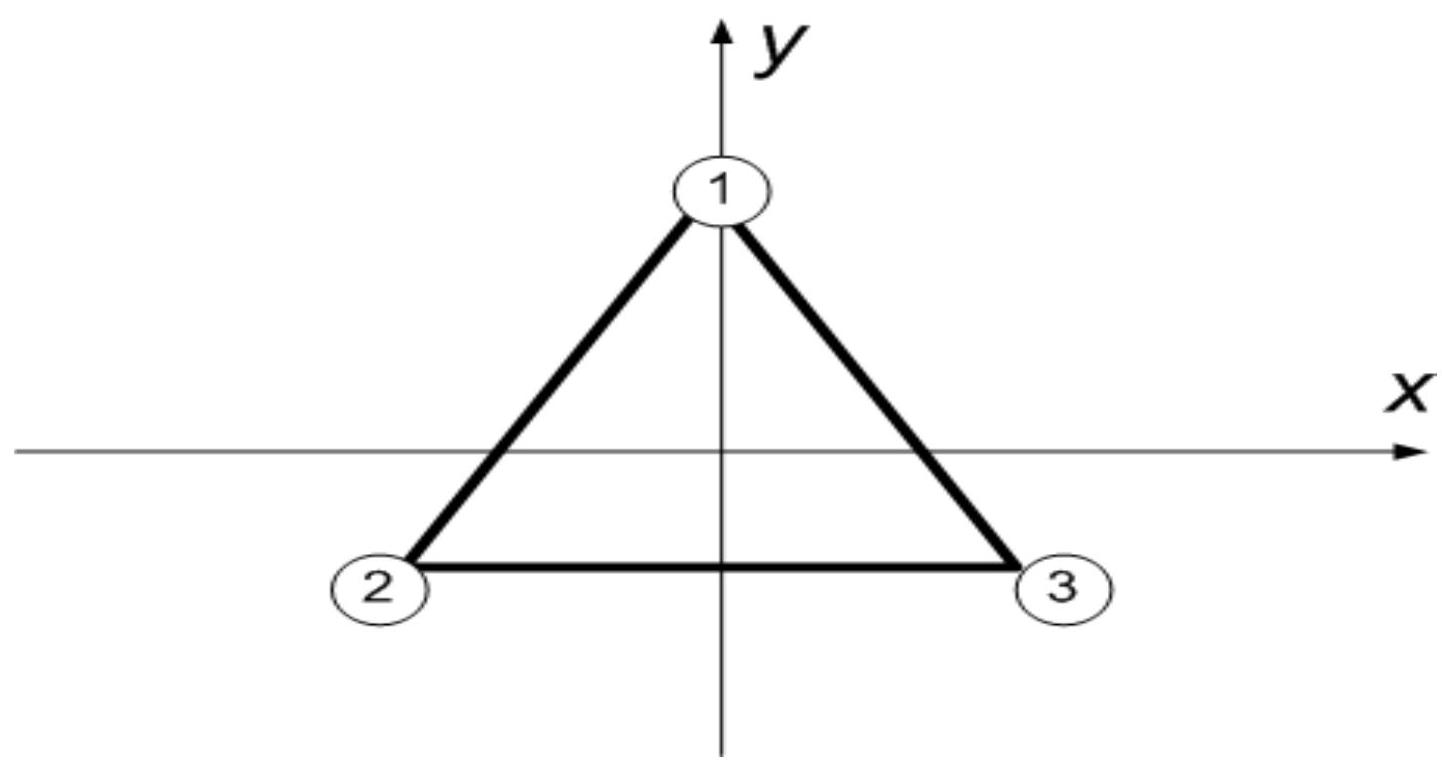
\includegraphics[max width=\textwidth]{2023_10_07_53b70c7408bc8e139415g-66(1)}
\end{center}

Fig 4.1: Desired formation of three WAM-Vs

\begin{center}
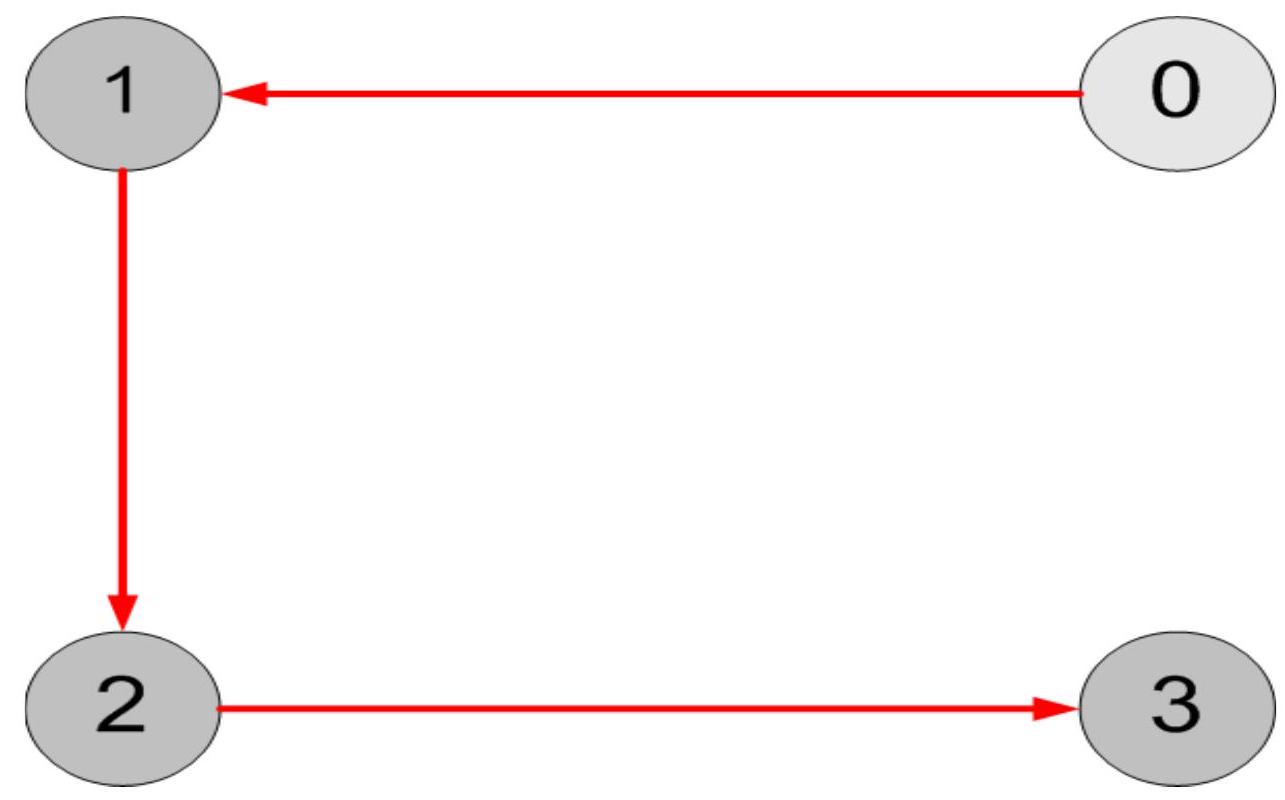
\includegraphics[max width=\textwidth]{2023_10_07_53b70c7408bc8e139415g-66}
\end{center}

Fig. 4.2: Communication digraph

\begin{center}
\includegraphics[max width=\textwidth]{2023_10_07_53b70c7408bc8e139415g-67(1)}
\end{center}

Fig 4.3: Time response of $\bar{x}_{j}$ for $1 \leq j \leq 3$

\begin{center}
\includegraphics[max width=\textwidth]{2023_10_07_53b70c7408bc8e139415g-67}
\end{center}

Fig 4.4: Time response of $\bar{y}_{j}$ for $1 \leq j \leq 3$

\begin{center}
\includegraphics[max width=\textwidth]{2023_10_07_53b70c7408bc8e139415g-68}
\end{center}

Fig 4.5: Time response of $z_{1 j}$ for $1 \leq j \leq 3$

\begin{center}
\includegraphics[max width=\textwidth]{2023_10_07_53b70c7408bc8e139415g-68(1)}
\end{center}

Fig. 4.6: Time response of $z_{2 j}$ for $1 \leq j \leq 3$

\begin{center}
\includegraphics[max width=\textwidth]{2023_10_07_53b70c7408bc8e139415g-69}
\end{center}

Figure 4.7: Time response of $z_{3 j}$ for $1 \leq j \leq 3$

\subsection{Conclusion}
In this Chapter, we considered formation control of multiple uncertain WAM-Vs with a leader WAM-V. If inertia parameters are not exactly known, distributed robust tracking laws were proposed with the aid of neighbors' information. To reduce the computation load in controller design, distributed command filtered controllers were proposed. Simulation results show the effectiveness of the proposed results.

\section{CHAPTER V}
\section{CONCLUSION AND FUTURE RESEARCH}
In this dissertation, we presented a distributed formation control strategy for a team of UAVs to autonomously achieve and maintain a desired formation while traveling toward a desired destination. Given a desired formation, we showed how stabilizing control gains can be found from solving a convex optimization problem. These gains, which can be communicated to the agents before start of the mission, were used to calculate linear and angular velocity control commands for the UAVs under the Dubins constraint. Simulations were provided to show that under the proposed control the UAVs achieve the desired formation and travel along the assigned direction. Proof of convergence for the saturated UAV control is a topic of future work. To preserve connectivity, avoid obstacles, or prevent collision among UAVs, distributed techniques such as potential field traffic circle or control barrier function approach can be employed. Another strategy is a temporary change of altitude, i.e., UAVs passing over or under each other to avoid collision. This strategy can preserve the stability properties, however, the low-level altitude controller can become more complicated. Incorporating collision/obstacle avoidance strategies with the proposed formation control and analyzing the stability properties of the resulting system will be a topic of future work. Again, we considered formation control of multiple uncertain WAM-Vs with a leader WAM-V. If inertia parameters are not exactly known, distributed robust tracking laws were proposed with the aid of neighbors' information. To reduce the computation load in controller design, distributed command filtered controllers were proposed. Simulation results show the effectiveness of the proposed results.

Lastly, we presented a distributed formation control strategy for a team of agents with a variety of dynamics to autonomously achieve a desired planar formation. Under the assumption that the sensing graph is undirected and universally rigid, we showed that formation control gains can be designed by solving a SDP problem. This design enjoys several robustness properties, such as robustness to positive scaling and rotation (up to $\pm 90^{\circ}$ ) of the control vector, saturations in the input, and switches in the sensing topology. The control was extended to agents with higher-order linear (or linearizable) holonomic dynamics, such as quadrotors, followed by further extension to agents with nonholonomic unicycle and car dynamics. An important outcome of this work was a fully distributed collision avoidance algorithm that emerged naturally from the robustness properties of the proposed strategy. To symplify the control, simulations for vehicles with different dynamics were presented, and experiments on a distributed robotic platform where performed.

Future work includes investigating additional requirements, such as inter-agent communication, to guarantee that the collision avoidance algorithm can overcome gridlock scenarios. Moreover, inter-agent communication can be exploited in a distributed optimization scheme to solve the SDP problem in a decentralized way. Other possible research avenues include extending the proposed approach to 3D formations.

\section{REFERENCES}
Z. Lin, L. Wang, Z. Han, and M. Fu, "Distributed formation control of multi-agent systems using complex laplacian," IEEE Transactions on Automatic Control, vol. 59, no. 7, pp. 17651777, July 2014

K. Fathian, D. I. Rachinskii, M. W. Spong, and N. R. Gans, "Globally asymptotically stable distributed control for distance and bearing basedmulti-agent formations," in American Control Conference. IEEE, 2016, pp. 4642-4648.

Z. Wang and M. Schwager, "Kinematic multi-robot manipulation with no communication using force feedback," in International Conference on Robotics and Automation. IEEE, 2016, pp. 427-432.

D. Saldana, B. Gabrich, M. Whitzer, A. Prorok, M. F. Campos, M. Yim, and V. Kumar, "A decentralized algorithm for assembling structures with modular robots," in International Conference on Intelligent Robots and Systems. IEEE, 2017, pp. 2736-2743.

R. Bähnemann, D. Schindler, M. Kamel, R. Siegwart, and J. Nieto, “A decentralized multi-agent unmanned aerial system to search, pick up, and relocate objects," in IEEE International Symposium on Safety, Security and Rescue Robotics, Oct 2017, pp. 123-128.

P. Rudol and P. Doherty, "Human body detection and geolocalization for uav search and rescue missions using color and thermal imagery," in Aerospace Conference, IEEE,2008, pp. 1-8.

M. A. Goodrich, B. S. Morse, D. Gerhardt, J. L. Cooper, M. Quigley, J. A. Adams, and C. Humphrey, "Supporting wilderness search and rescue using camera-equipped mini uav," Journal of Field Robotics, vol. 25, no. 1-2, pp. 89-110, 2008.

K. M. Fornace, C. J. Drakeley, T. William, F. Espino, and J. Cox, "Mapping infectious disease landscapes: unmanned aerial vehicles and epidemiology," Trends in parasitology, vol. 30, no. 11, pp. 514-519,2014.

J. Zhang, J. Hu, J. Lian, Z. Fan, X. Ouyang, and W. Ye, "Seeing them forest from drones: Testing the potential of lightweight drones as a tool for long-term forest monitoring," Biological Conservation, vol. 198, pp. 60-69, 2016.

K. Fathian, D. I. Rachinskii, M. W. Spong, and N. R. Gans, "Globally asymptotically stable distributed control for distance and bearing based multi-agent formations," in American Control Conference. IEEE, 2016, pp. 4642-464 Z. Yan, N. Jouandeau, and A. A. Cherif, "A survey and analysis of multi-robot coordination," International Journal of Advanced Robotic Systems, vol. 10, no. 12, p. 399,2013.

K.-K. Oh, M.-C. Park, and H.-S. Ahn, “A survey of multi-agent formation control,” Automatica, vol. 53, pp. 424440, 2015.

N. Michael, M. M. Zavlanos, V. Kumar, and G. J. Pappas, "Distributed multi-robot task assignment and formation control," in International Conference on Robotics and Automation. IEEE, 2008, pp. 128-133.

N.-s. P. Hyun, P. A. Vela, and E. I. Verriest, "Collision free and permutation invariant formation control using the root locus principle," in American Control Conference. IEEE, 2016, pp. 2572-2577.

T. Motoyama and K. Cai, "Top-down synthesis of multi-agent formation control: An eigenstructure assignment-based approach," in American Control Conference. IEEE, 2017, pp. 259-264.

E. Montijano, D. Zhou, M. Schwager, and C. Sagues, "Distributed formation control without a global reference frame," in American Control Conference. IEEE, 2014, pp. 3862-3867.

S. Zhao and D. Zelazo, "Bearing rigidity and almost global bearingonly formation stabilization," IEEE Transactions on Automatic Control, vol. PP, no. 99, pp. 1 - 1,2015.

M.-C. Park, Z. Sun, B. D. Anderson, and H.-S. Ahn, "Distancebased control of Kn formations in general space with almost global convergence," IEEE Transactions on Automatic Control, 2017.

A. Weinstein, A. Cho, G. Loianno, and V. Kumar, "Visual inertial odometry swarm: An autonomous swarm of vision-based quadrotors" IEEE Robotics and Automation Letters, vol. 3, no. 3, pp. $1801-1807$, July 2018.

M. Aranda, G. López-Nicolás,C. Sagüés, and M. M. Zavlanos, "Coordinate-free formation stabilization based on relative position measurements," Automatica, vol. 57, pp. 11 20,2015 .

R. Olfati-Saber and R. M. Murray, "Distributed cooperative control of multiple vehicle formations using structural potential functions," in IFAC World Congress, 2002, pp. 346352.

L. Krick, M. E. Broucke, and B. A. Francis, "Stabilisation of infinitesimally rigid formations of multi-robot networks," International Journal of Control, vol. 82, no. 3, pp. 423-439, 2009

\section{BIOGRAPHICAL SKETCH}
Md Nur-A-Adam Dony was born in Rajshahi, Bangaldesh on January $1^{\text {st }}, 1995$. On October 25, 2016, he completed a Bachelor of Science in Electrical Engineering from the Rajshahi University of Engineering \& Technology. He moved to USA to Pursue his Master's degree in August,2019 with full scholarship. As a graduate student, Dony had the opportunity to work on his research as graduate research assistant, where he began his research on Control of unmanned aerial vehicles (UAV).He published 3 research papers during his masters study. Lastly, he worked as a graduate teaching assistant for the following course areas: Automatic Control, Communication Network. He was awarded a Master of Science in Engineering from the University of Texas Rio Grande Valley in May of 2021.

1709 W Schunior St, Edinburg, TX,78541

Email: \href{mailto:nuraadamdonyeeeruet11@gmail.com}{nuraadamdonyeeeruet11@gmail.com}


\end{document}